% !TeX root = ../dokumentation.tex

\chapter{Technische Umsetzung}


\section{Architektur}
Um unsere Plattform potenziellen Nutzern zugänglich zu machen und bestimmte Teile unseres Workflows\footnote{Arbeitsablauf} zu Automatisieren, hosten wir unsere Architektur in einer Cloud Umgebung.
Dabei läuft unsere Architektur auf der Kontainer Orchestrierungs Plattform Kubernetes, für welches wir die leichgewichtige (und leichter zu verwaltende) Variante \textit{k3s}~\parencite{web/k3s} verwenden.
Auf diesem Kubernetes System werden \ac{CI/CD} Plattformen gehosted und unsere Applikation sowie deren Abhängigkeiten. Dadruch sind wir nicht an öffentlich-kostenfreie System limitiert und können unsere
System perfekt auf unseren Workflow und die Applikation anpassen.

\subsection{Übersicht der Services}
Unser Produkt ist in mehrere Services aufgeteilt. Die Services sind \textit{Core-Service}, \textit{Polling-Service} und das \textit{Frontend}.
Desweiteren gibt es eine \textit{PostgreSQL Datenbank} und eine \textit{Keycloak} Instanz. Die letzten beiden Services sind Abhänigkeiten von unseren entwickelten Services.
Die Datenbank wird dafür verwendet um Daten wie RSS-Feeds und Artikel zu speichern.
Keycloak wird dafür verwendet um den \textit{Core-Service} und das \textit{Frontend} abzusichern und die Benutzer zu verwalten.
Die Hauptaufgabe des \textit{Core-Services} ist es RSS-Feeds und Artikel zur Verfügung zu stellen, dies geschieht mittels \textit{GraphQL}. Desweiteren bietet er die Möglichkeit
RSS-Feeds anzulegen und Abonnents, Favouriten und Lesezeichen eines Benutzers zu verwalten.
Der \textit{Polling-Service} ist für die automatische Datenabfrage von RSS-Feeds und deren Artikel zuständig. Diese werden anschließend in der Datenbank gespeichert.
Das \textit{Frontend} ist die Endschnittstelle unseres Produkts zu dem Benutzer.
Es wird dafür verwendet um die Daten des \textit{Core-Services} dem Benutzer zugänglich zu machen.
Das folgenden Diagramm veranschautlicht die Skiosa Service-Architektur. Die Sevices mit den gestrichelten Linien sind die Abhängigkeiten.
\begin{figure}[!htbp]
    \centering    
    \usetikzlibrary{positioning}
    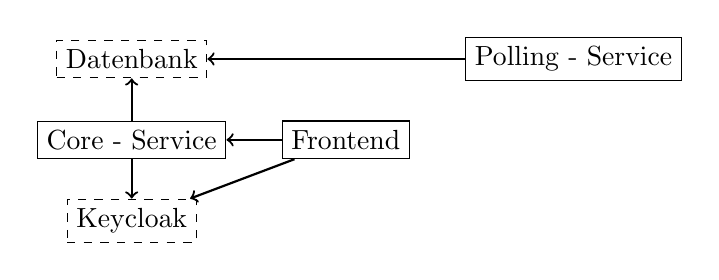
\begin{tikzpicture}
        \matrix [column sep=7mm, row sep=5mm] {
            \node (database) [draw, shape=rectangle, dashed] {Datenbank}; &&
            \node (polling_service) [draw, shape=rectangle] {Polling - Service}; \\
            \node (core_service) [draw, shape=rectangle] {Core - Service}; &
            \node (frontend) [draw, shape=rectangle] {Frontend}; \\
            \node (keycloak) [draw, shape=rectangle, dashed] {Keycloak}; \\
            };
            \draw[->, thick] (core_service) -- (database);
            \draw[->, thick] (frontend) -- (core_service);
            \draw[->, thick] (polling_service) -- (database);
            \draw[->, thick] (core_service) -- (keycloak);
            \draw[->, thick] (frontend) -- (keycloak);
        \end{tikzpicture}        
\caption{Diagramm – Darstellung der Service Architektur}
\end{figure}

\subsection{CI/CD Infrastrukture}
Um Code Qualität zu gewährleisten, wurde eine \ac{CI/CD} Infrastruktur entwickelt.
Diese ermöglicht es uns automatisiert Tests wie Unit und Integration Tests auszuführen und nach jeder Änderung aktuelle Versionen der Software zu veröffentlichen.
Da zum Beispiel eine neue veröffentlichung bei Änderungen auf der Master Branch stattfinden sollen, gibt es drei verschieden \ac{CI/CD} Pipelines.
Eine die nur Unit-Tests ausführt, eine die komplexe Tests ausführt und eine die eine neue Version veröffentlicht.

\subsubsection{Übersicht der Standard \ac{CI}-Pipline}
Die Standard \ac{CI}-Pipeline wird bei jedem Commit der nicht auf dem Master Branch stattfindet ausgeführt. Dabei hat die Standard Pipeline den geringsten Umfang and Aufgaben.
Diese führt nur die Unit-Tests aus, dazu muss der Code gecloned und alle Dependencies installiert werden. Somit sind direkt Fehler schon früh erkennbar, wenn diese Pipeline fehlschlägt.
\begin{figure}[!htbp]
    \centering    
    \usetikzlibrary{positioning}
    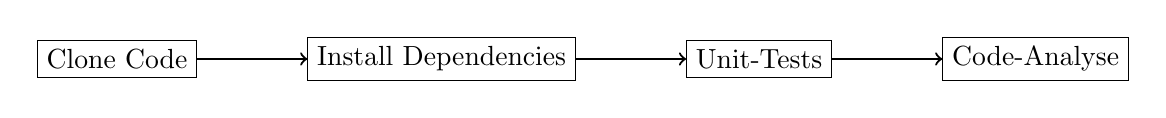
\begin{tikzpicture}
        \matrix [column sep=7mm, row sep=5mm] {
            \node (clone) [draw, shape=rectangle] {Clone Code}; &&
            \node (npm_setup) [draw, shape=rectangle] {Install Dependencies}; &&
            \node (unit_test) [draw, shape=rectangle] {Unit-Tests}; &&
            \node (sonar) [draw, shape=rectangle] {Code-Analyse}; \\
            };
            \draw[->, thick] (clone) -- (npm_setup);
            \draw[->, thick] (npm_setup) -- (unit_test);
            \draw[->, thick] (unit_test) -- (sonar);
        \end{tikzpicture}        
\caption{Diagramm – Darstellung der Standard \ac{CI}-Pipeline}
\end{figure}

\subsubsection{Übersicht der Pull-Request \ac{CI}-Pipline}
Die Pull-Request \ac{CI}-Pipeline wird ausgeführt sobald ein Pull-Request erstellt wird. Ihr Ziel ist es den jeweiligen Reviewer zu unterstützen, indem sie Tests und Code-Analyse durchführt.
Die Ergebnisse der Code Analyse werden direkt auf der Pull-Request Seite dargestellt. Sollten diese nicht den mindestanforderungen entsprechen, wird der Pull-Request dadurch blockiert.
Die Pipeline beinhaltet die selben Schritte wie die Standard Pipeline, sie erweitert diese lediglich um Integration-Tests.
\begin{figure}[!htbp]
    \centering    
    \usetikzlibrary{positioning}
    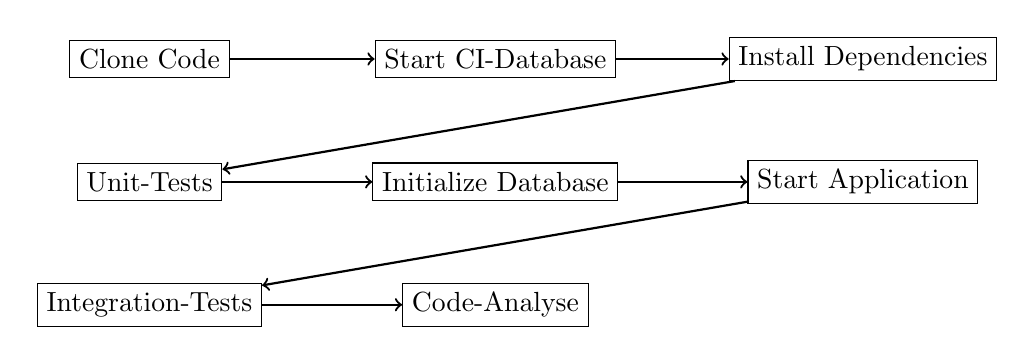
\begin{tikzpicture}
        \matrix [column sep=7mm, row sep=10mm] {
            \node (clone) [draw, shape=rectangle] {Clone Code}; &&
            \node (database) [draw, shape=rectangle] {Start \ac{CI}-Database}; &&
            \node (npm_setup) [draw, shape=rectangle] {Install Dependencies}; \\
            \node (unit_test) [draw, shape=rectangle] {Unit-Tests}; &&
            \node (init_db) [draw, shape=rectangle] {Initialize Database}; &&
            \node (start_app) [draw, shape=rectangle] {Start Application}; \\
            \node (int_test) [draw, shape=rectangle] {Integration-Tests}; &&
            \node (sonar) [draw, shape=rectangle] {Code-Analyse}; \\
            };
            \draw[->, thick] (clone) -- (database);
            \draw[->, thick] (database) -- (npm_setup);
            \draw[->, thick] (npm_setup) -- (unit_test);
            \draw[->, thick] (unit_test) -- (init_db);
            \draw[->, thick] (init_db) -- (start_app);
            \draw[->, thick] (start_app) -- (int_test);
            \draw[->, thick] (int_test) -- (sonar);
        \end{tikzpicture}
\caption{Diagramm – Darstellung der Pull-Request \ac{CI}-Pipeline}
\end{figure}

\subsubsection{Übersicht der Master \ac{CI}-Pipline}
Die Master \ac{CI}-Pipeline wird bei einen Commit auf den Master Branch ausgeführt. Dabei hat die Pipeline die Aufgabe den neuen Code auszurollen und sommit live zu bringen.
Zur Sicherheit werden auch wieder die Unit-Tests ausgeführt, damit auch wirklich sichergestellt wird, dass der Code lauffähig ist. Anschließend wird ein neues Docker-Image gebaut
welches dann in der Docker-Registry gespeichert wird. Nach erfolgreichem bauen des Images, wird die neue Image-Version in das Kubernetes-Depyoment geschrieben. Denn ArgoCD~\parencite{web/argocd} unser \ac{CD} Tool
erkennt automatisch Änderungen an den Kubernetes-Deployments und übernimmt diese. Somit sind die Code Änderungen an der Software in wenigen Minuten live ausgerollt.
\begin{figure}[!htbp]
    \centering    
    \usetikzlibrary{positioning}
    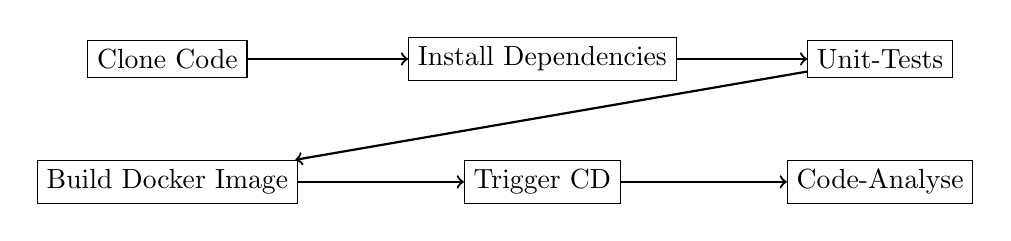
\begin{tikzpicture}
        \matrix [column sep=7mm, row sep=10mm] {
            \node (clone) [draw, shape=rectangle] {Clone Code}; &&
            \node (npm_setup) [draw, shape=rectangle] {Install Dependencies}; &&
            \node (unit_test) [draw, shape=rectangle] {Unit-Tests}; \\
            \node (docker_build) [draw, shape=rectangle] {Build Docker Image}; &&
            \node (trigger_cd) [draw, shape=rectangle] {Trigger \ac{CD}}; &&
            \node (sonar) [draw, shape=rectangle] {Code-Analyse}; \\
            };
            \draw[->, thick] (clone) -- (npm_setup);
            \draw[->, thick] (npm_setup) -- (unit_test);
            \draw[->, thick] (unit_test) -- (docker_build);
            \draw[->, thick] (docker_build) -- (trigger_cd);
            \draw[->, thick] (trigger_cd) -- (sonar);
        \end{tikzpicture}
\caption{Diagramm – Darstellung der Master \ac{CI}-Pipeline}
\end{figure}

\section{Mockups}
\subsection{Design Language}
Im Projekt haben wir mit dem Ziel eines einheitlichen Designs eine Design-Language definiert.
Eine Design-Language kann als Framework verstanden werden, das es Teams ermöglicht, 
zusammenhängende Schnittstellen zu erstellen und zu entwerfen um Anwendungen ein \enquote{einzigartiges Gefühl} zu verleihen.
Im engeren Sinne kann eine Design-Language als Set von Regeln, die Typografie, Formen und Muster vorschreiben.

Zur Maximierung der Vorteile eines solchen Systems in unserem Projekt wurden folgende Ziele und Ideen genutzt:
\begin{itemize}
    \item Skiosa ein kohärentes Erscheinungsbild zu geben, das mit dem Branding übereinstimmt und so den wahrgenommenen Wert unseres Projekts verbessert.
    \item Visuelle Trennung der verschiedenen Interessenebenen (z. B. Inhalt, Einstellungen, Navigation)
    \item Klar anzugeben, welche Teile der Benutzeroberfläche von Skiosa sind und welche von externen Quellen stammen.
\end{itemize}

Als Schriftart soll für primäre Schaltflächen oder Texte \enquote{Pacifico} in Bold verwendet werden.
Für zusätzliche \enquote{Helper Texte} wie Menüpunkte, Schaltflächen oder Untertitel sollte \enquote{Ubuntu Mono} in Bold genutzt werden.

In SKIOSA gibt es drei Arten von Content.  
\begin{itemize}
    \item Side bar (split top bar on mobile) mit wichtigen Inhalten
    \item Main Content
    \item Meta Content
\end{itemize}

Damit Nutzer Content besser unterscheiden zu können, wird das Design dieser drei Items unterschiedlich sein.

\textbf{Side bar:}
\begin{itemize}
    \item Dunklere (oder umgekehrte) Färbung, um sie hervorzuheben
    \item Das Skiosa Logo wird immer oben angezeigt
\end{itemize}

\textbf{Main Content}
\begin{itemize}
    \item Besteht aus einzelnen Karten auf dunklerem Hintergrund, ohne Schatten
    \item Einzelne Karten enthalten optionale \enquote{Untertitel} zur Erläuterung ihres Sinns
    \item Wenn eine Seite eine Überschrift hat, wird diese zusammen mit einer Beschreibung oder anderen Metadaten die oberste Kachel bilden (Ausnahmen sind Seiten mit nur einer Kachel)
    \item Inhalt ist immer das farbigste Element der Seite und wechselt zwischen verschiedenen Farbtönen für verschiedene Elemente (vgl. Abbildung~\ref{fig:Page-Structure-Example})
\end{itemize}

\begin{figure}
    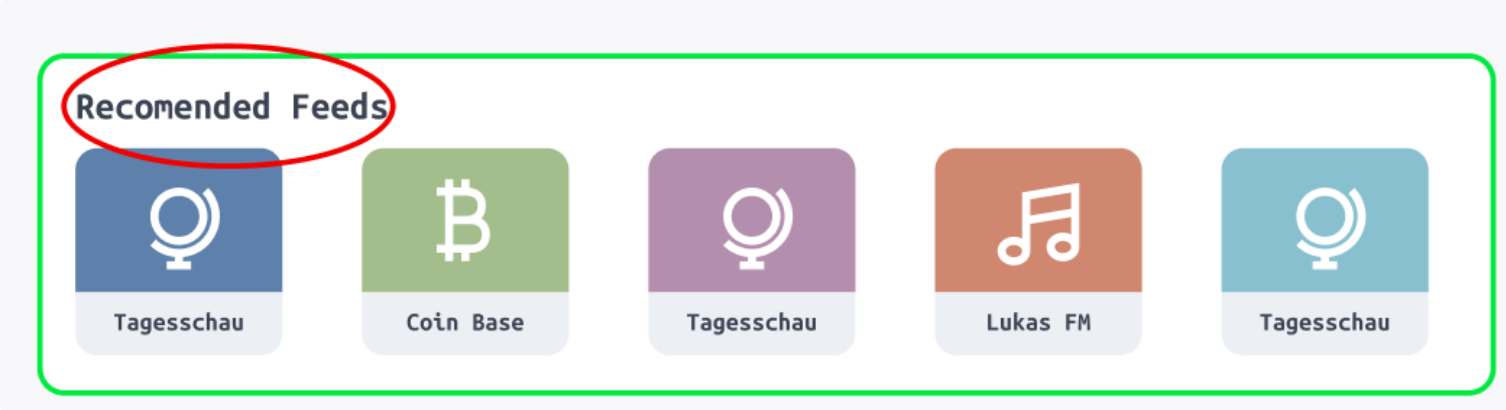
\includegraphics[width=\linewidth]{Page-Structure.png}
    \caption{Example for page structure (red: subtitle, green: card)}
    \label{fig:Page-Structure-Example}
\end{figure}

\textbf{Meta Content}
\begin{itemize}
    \item Seiten haben eine Karte
    \item Unterscheidet sich von normalen Seiten durch eine abgeschwächte Version der Seitenleiste
    \item Vermeidung von mehreren Farben (wie bei der obigen Feed)
\end{itemize}
 
\textbf{Formen}

Im Allgemeinen sollen Formen abgerundete Rechtecke mit einem Radius von 20px sein. Die Sidebar ist hier die Außnahme, da sie richtige Ecken hat, 
mit dem Ziel diese bewusst visuell vom restlichen Content abzugrenzen.
Buttons, Input-Felder, etc. sollen wie in Abbildung~\ref{fig:Design-Shapes-Example} aussehen. 
Dabei müssen Felder, die über mehrere Lines gehen, wie bspw. Listen, diese Regel nicht befolgen.

\begin{figure}[H]
    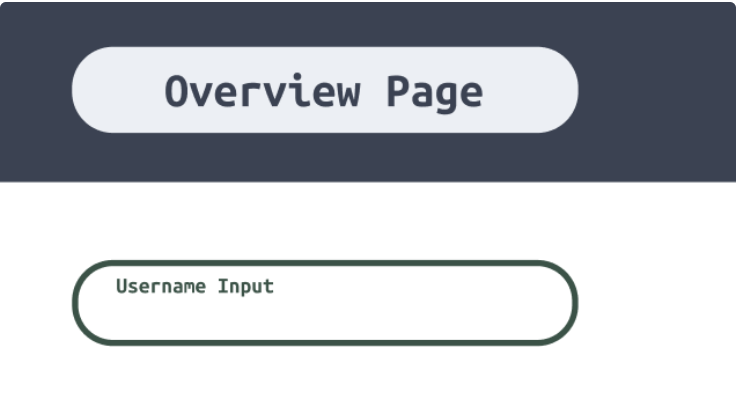
\includegraphics[width=\linewidth]{Design-Shapes-Example.png}
    \caption{Beispiel für Form von Buttons und Input-Feldern}
    \label{fig:Design-Shapes-Example}
\end{figure}

Bei der Angabe von Feldern, die andernfalls Inhalte oder Benutzerprofilbilder enthalten würden,
sollten wir allgemeine Symbole verwenden, die sich auf ihre Kategorie beziehen, um diese Lücke zu schließen.

\textbf{Farbschema}

In Skiosa wurde ein Farbschema festgelegt mit dem Ziel, 
eine möglichst einheitliche Nutzererfahrung zu ermöglichen. 
Dabei wird zwischen einem Dark-Mode und einem Light-Mode unterschieden (vgl. Abbildung~\ref{fig:Vergleich-light-dark}).
Für beide Modi wurden die Farben von Hintergründen und Artikelschriftart festgelegt.
Der Light- und Dark-Modus verwendet 
aber bei sonstigen Schriftfarben, Buttons, Eingabefeldern und Navigationshintergründen die selben Farben.

\begin{figure}[h]
    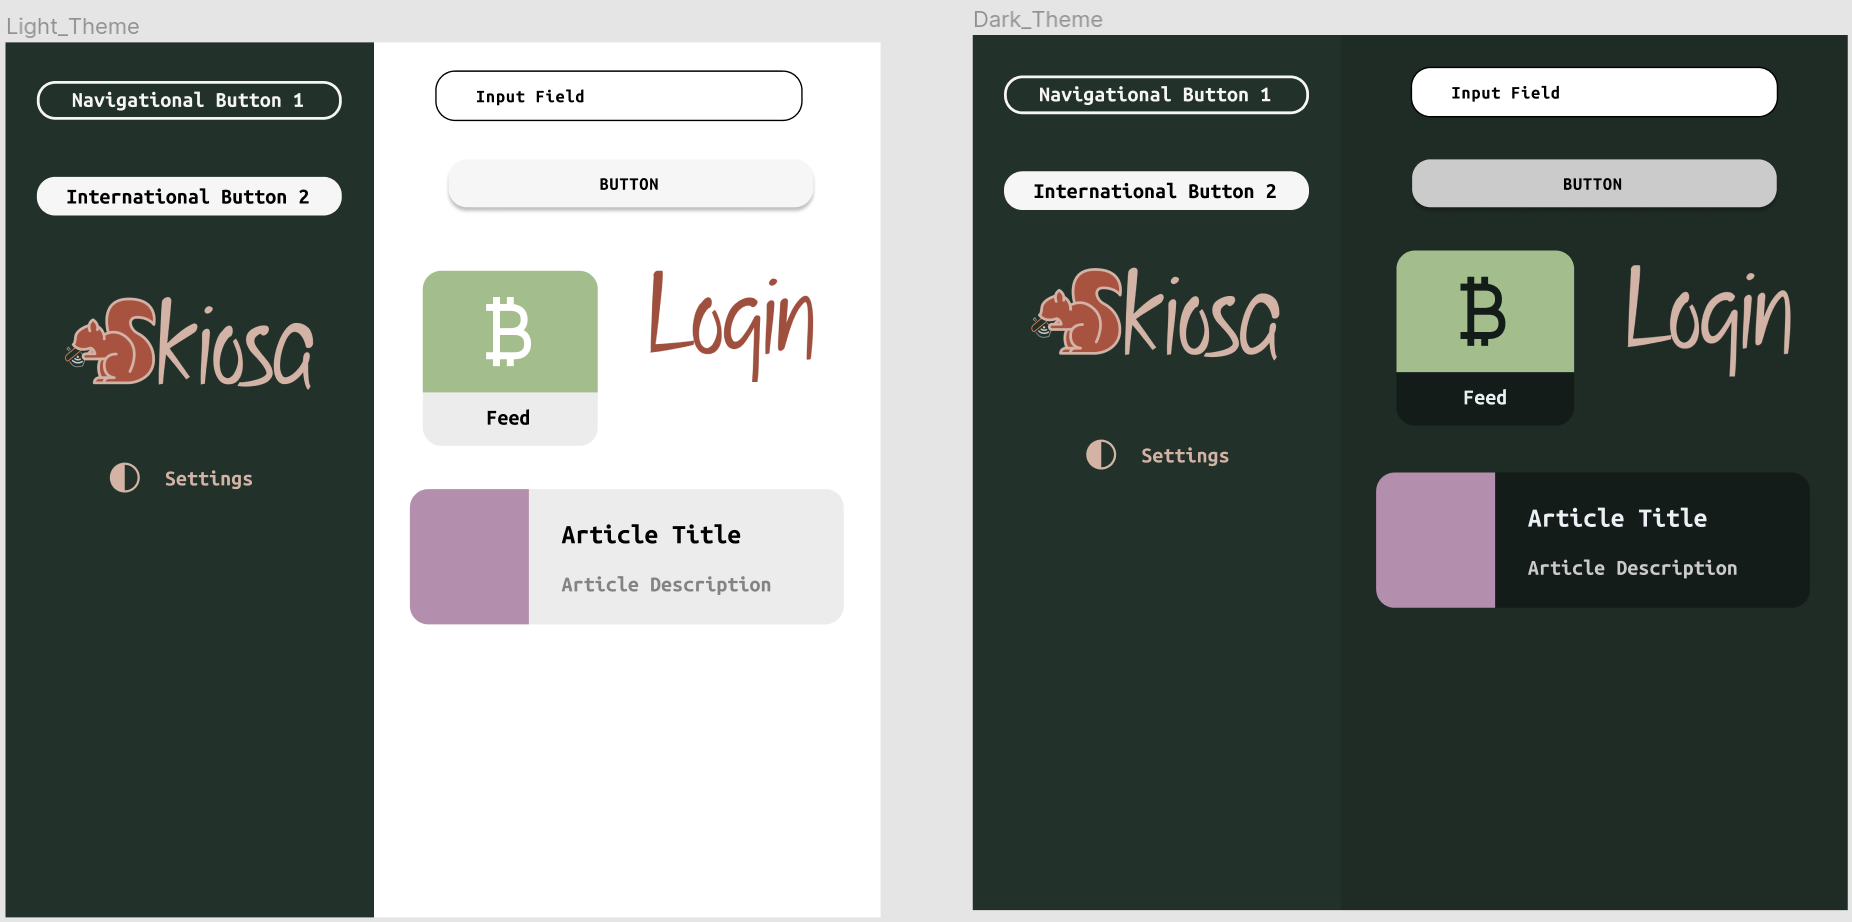
\includegraphics[width=\linewidth]{Vergleich-zwischen-light-und-dark-theme.png}
    \caption{Vergleich zwischen Light- und Dark-Modus in Skiosa}
    \label{fig:Vergleich-light-dark}
\end{figure}

\subsection{Nutzung von Figma}

Zur Erstellung des Designs und der Mockups wurde in Skiosa das Tool Figma verwendet. 
Für Komponenten die häufig verwendet werden sollen (bpsw. Buttons oder Farben) wurden sogenannte Common-Components erstellt.
Diese können bei der Erstellung von neuen Seiten wieder verwendet werden. 
Dadurch bleibt ein Button immer gleich und wird auch nur einmal in einem Angular-Component umgesetzt werden.
Ähnlich werden auch die Farben umgesetzt. 
Ziel ist es, effizienter neue Seiten erstellen zu können, die in das Design passen.

\subsection{Figma Designs}

Auf der Add-Feed-Page kann ein RSS-Feed für die Seite hinzugefügt werden. Mit dem Button \enquote{search} kann überprüft werden, ob die RSS-URL funktioniert.
Dabei kann einem RSS-Feed ein eigenden Namen und Beschreibung gegeben werden.(vgl. Abbildung~\ref{fig:Add Feed Desktop Light}) 
\begin{figure}[H]
    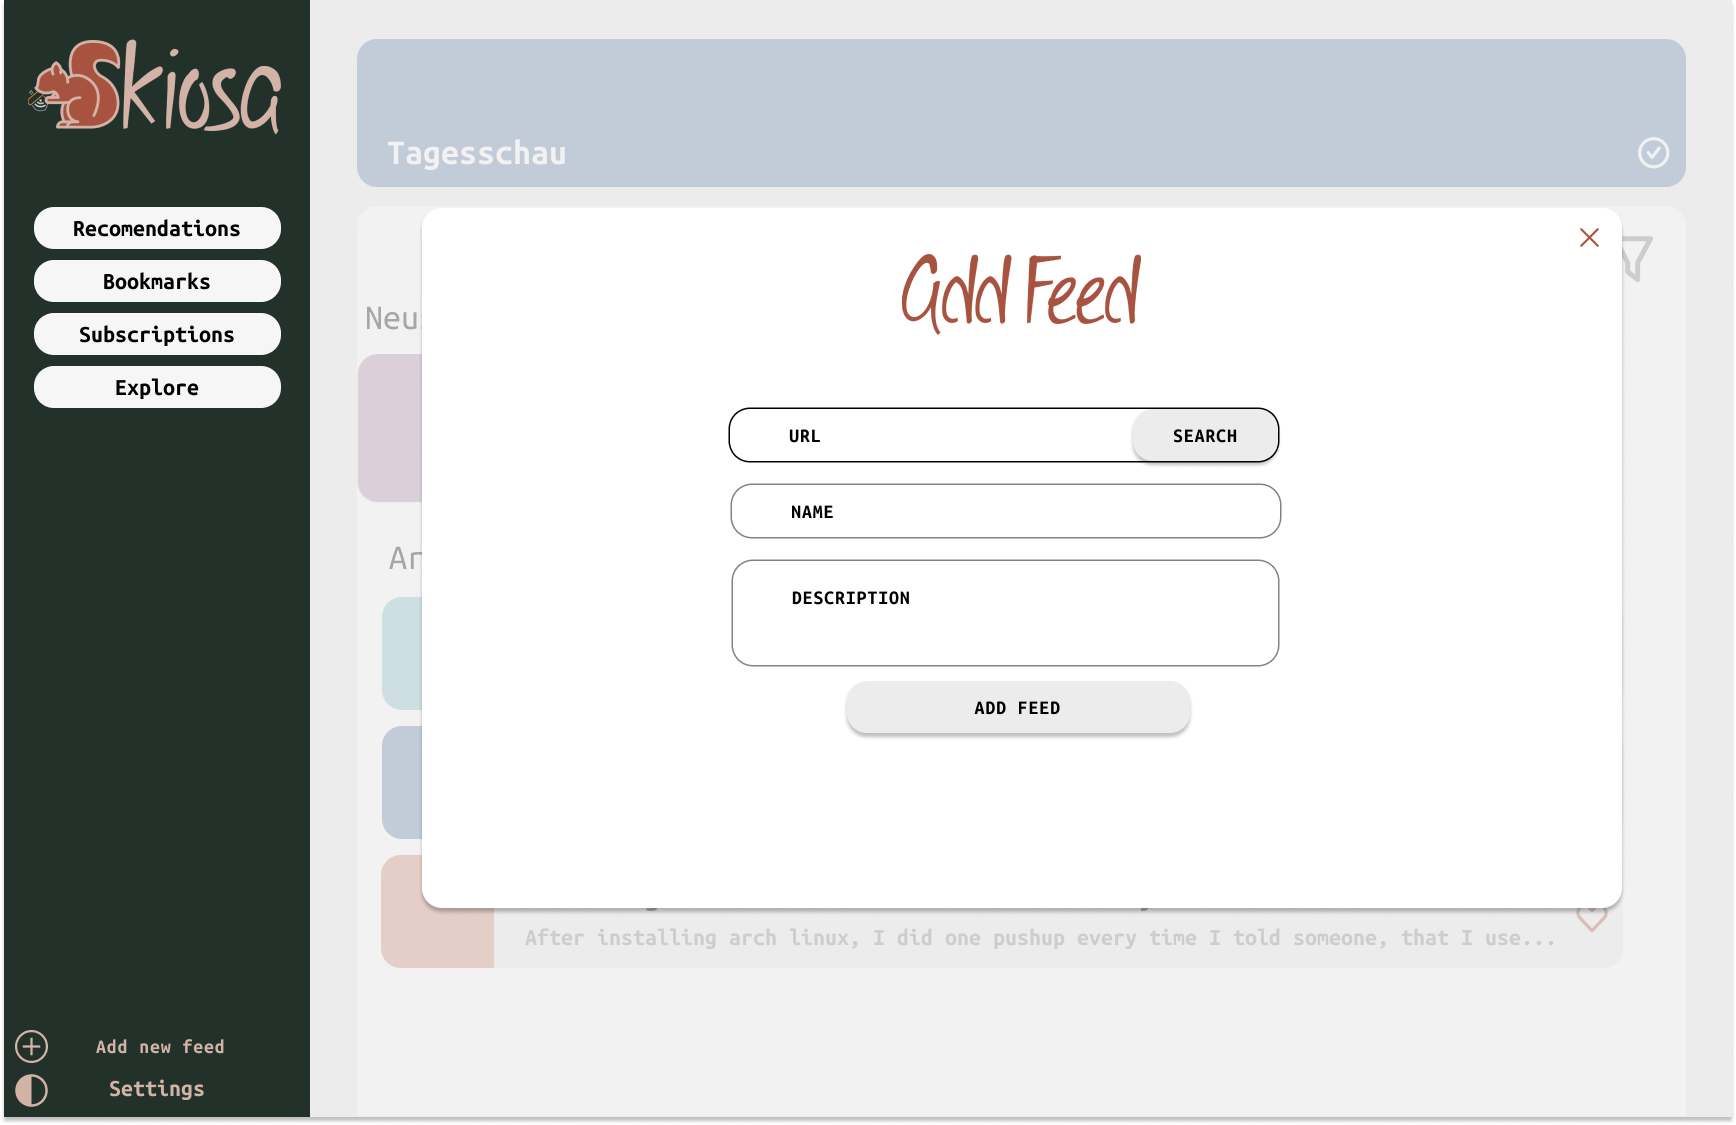
\includegraphics[width=\linewidth]{Add Feed Desktop Lightfigma-mockups.png}
    \caption{Mockup für Add-Feed-Page auf Desktop im Light-Mode}
    \label{fig:Add Feed Desktop Light}
\end{figure}

Auf der Bookmarks-Page werden alle bookmarked Artikel angezeit.
Dabei können diese Artikel noch zusätzlich geliked werden. (vgl. Abbildung~\ref{fig:Bookmarks Interface Desktop Light})

\begin{figure}[H]
    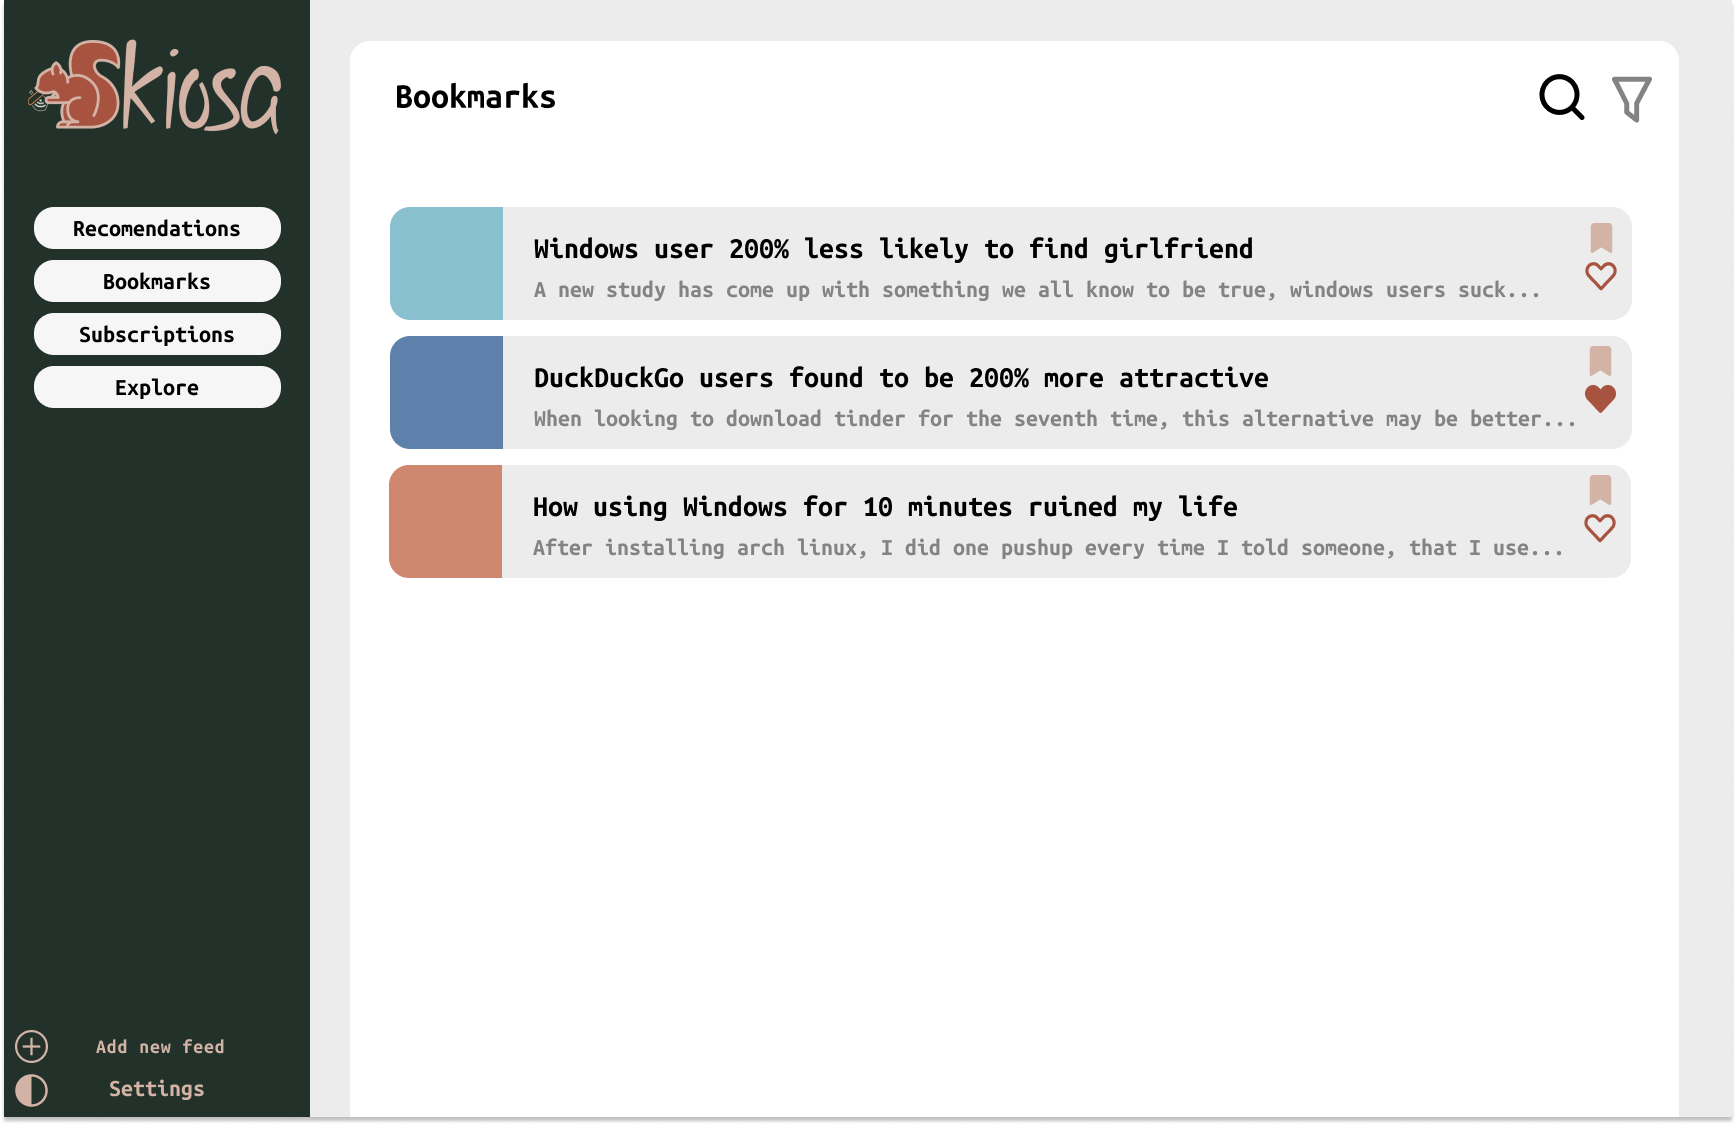
\includegraphics[width=\linewidth]{Bookmarks Interface Desktop Lightfigma-mockups.png}
    \caption{Mockup für Bookmark-Page auf Desktop im Light-Mode}
    \label{fig:Bookmarks Interface Desktop Light}
\end{figure}

Auf der Feed-Overview-Page werden von einem Feed sowohl die neusten Artkel als auch alternative Artikel aus dem Feed angezeigt.
Die Artikel können hier direkt sowohl geliked als auch bookmarked werden. (vgl. Abbildung~\ref{fig:Feed Overview Page Light Desktop})

\begin{figure}[H]
    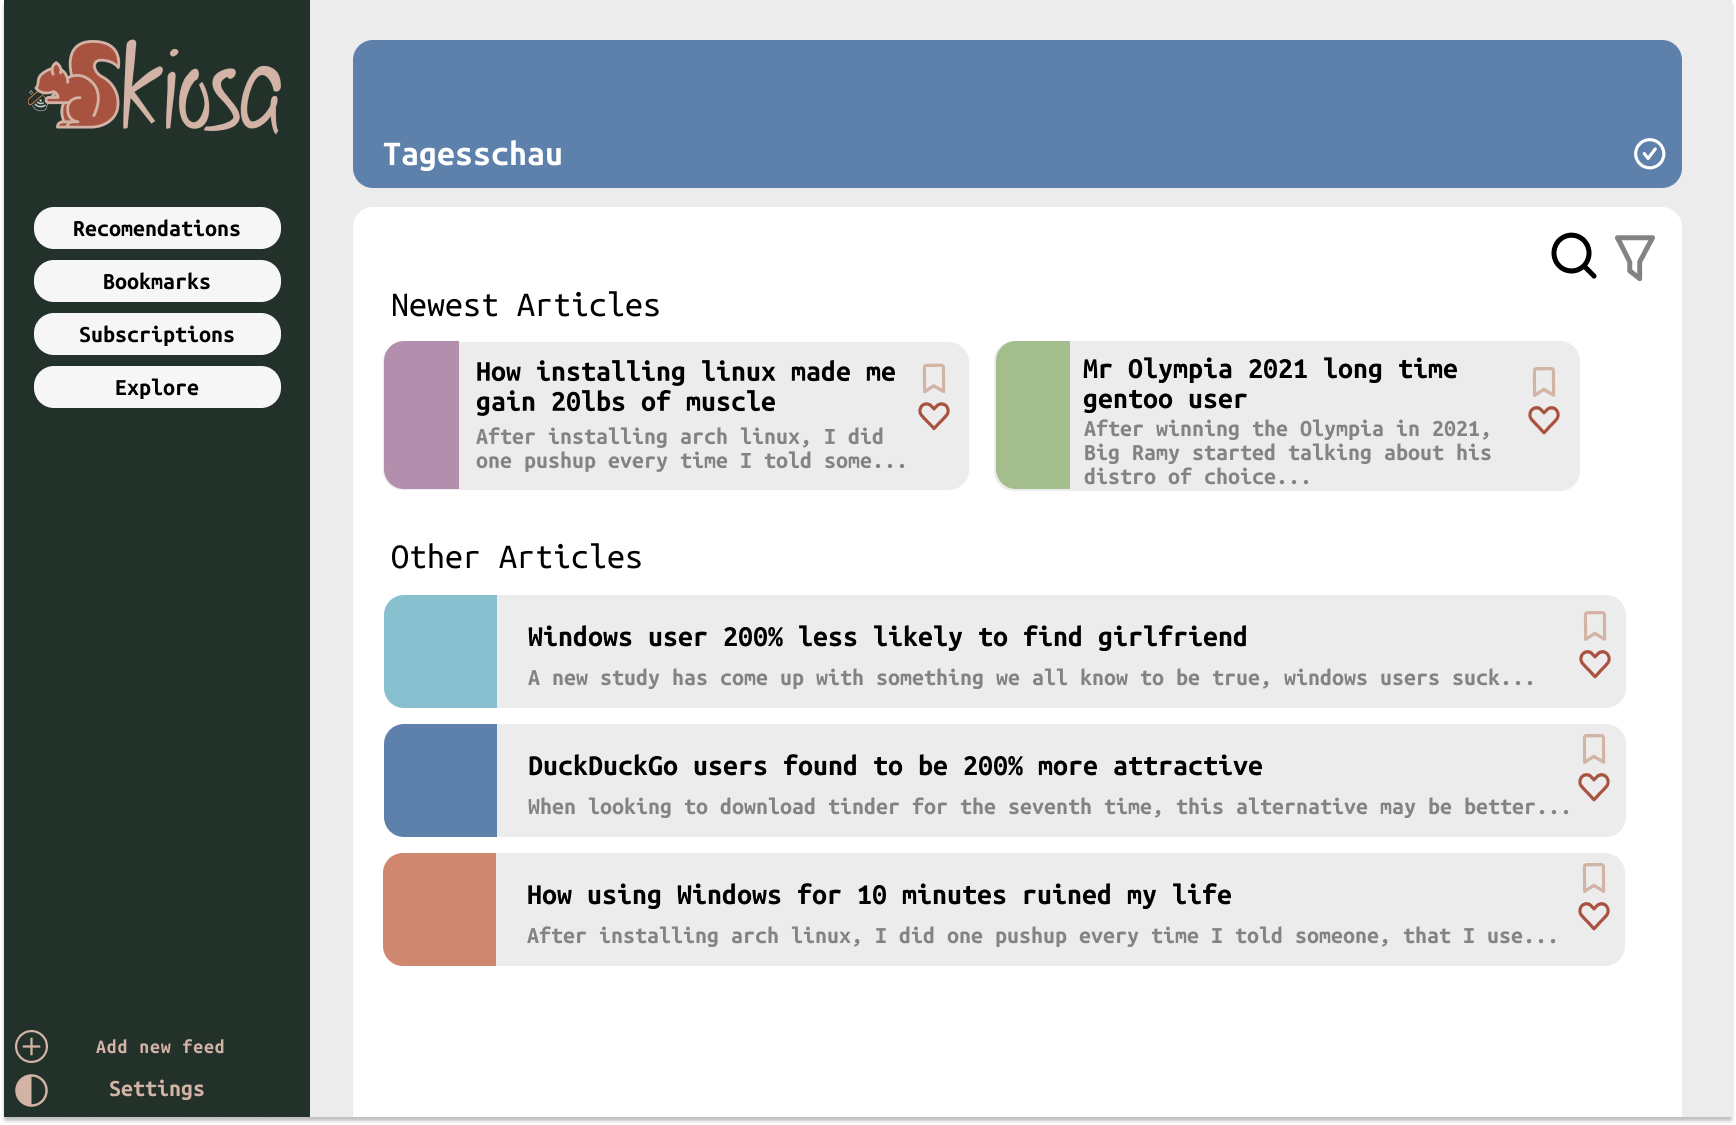
\includegraphics[width=\linewidth]{Feed Overview Page Desktop Lightfigma-mockups.png}
    \caption{Mockup für Feed-Overview-Page auf Desktop im Light-Mode}
    \label{fig:Feed Overview Page Light Desktop}
\end{figure}

Auf der Registrierungsseite wird der User nach dem 
Vornamen, Nachnamen, E-Mail-Adresse, Nutzername und nach seinem Passwort gefragt. Das Passwort muss dabei wiederhohlt werden. (vgl. Abbildung~\ref{fig:Registration Page Light})

\begin{figure}[H]
    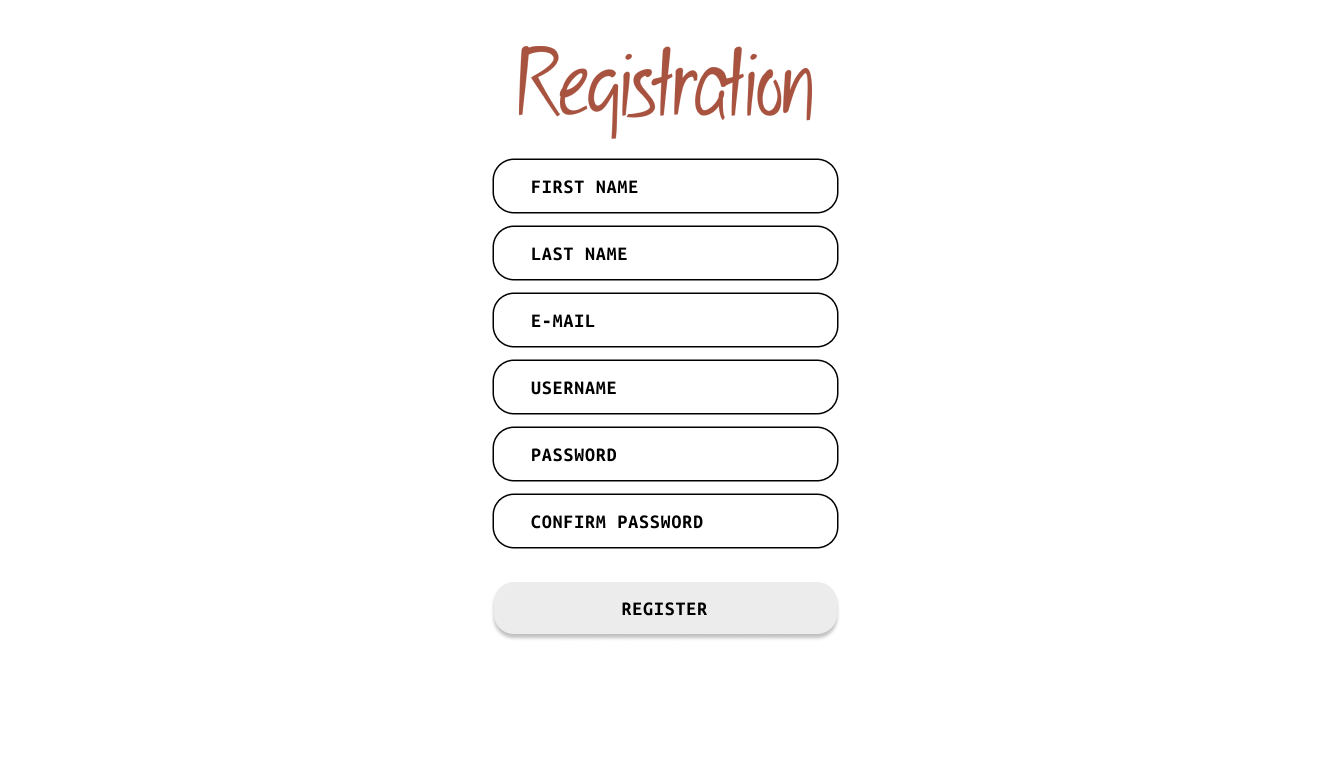
\includegraphics[width=\linewidth]{Framefigma-mockups-1.png}
    \caption{Mockup für Registration-Page auf Desktop im Light-Mode}
    \label{fig:Registration Page Light}
\end{figure}

Auf der Login-Page wird der User nach seinem Nutzername und Passwort gefragt, damit er auf der Seite angemeldet werden kann. (vgl. Abbildung~\ref{fig:Login Page Desktop Light})

\begin{figure}[H]
    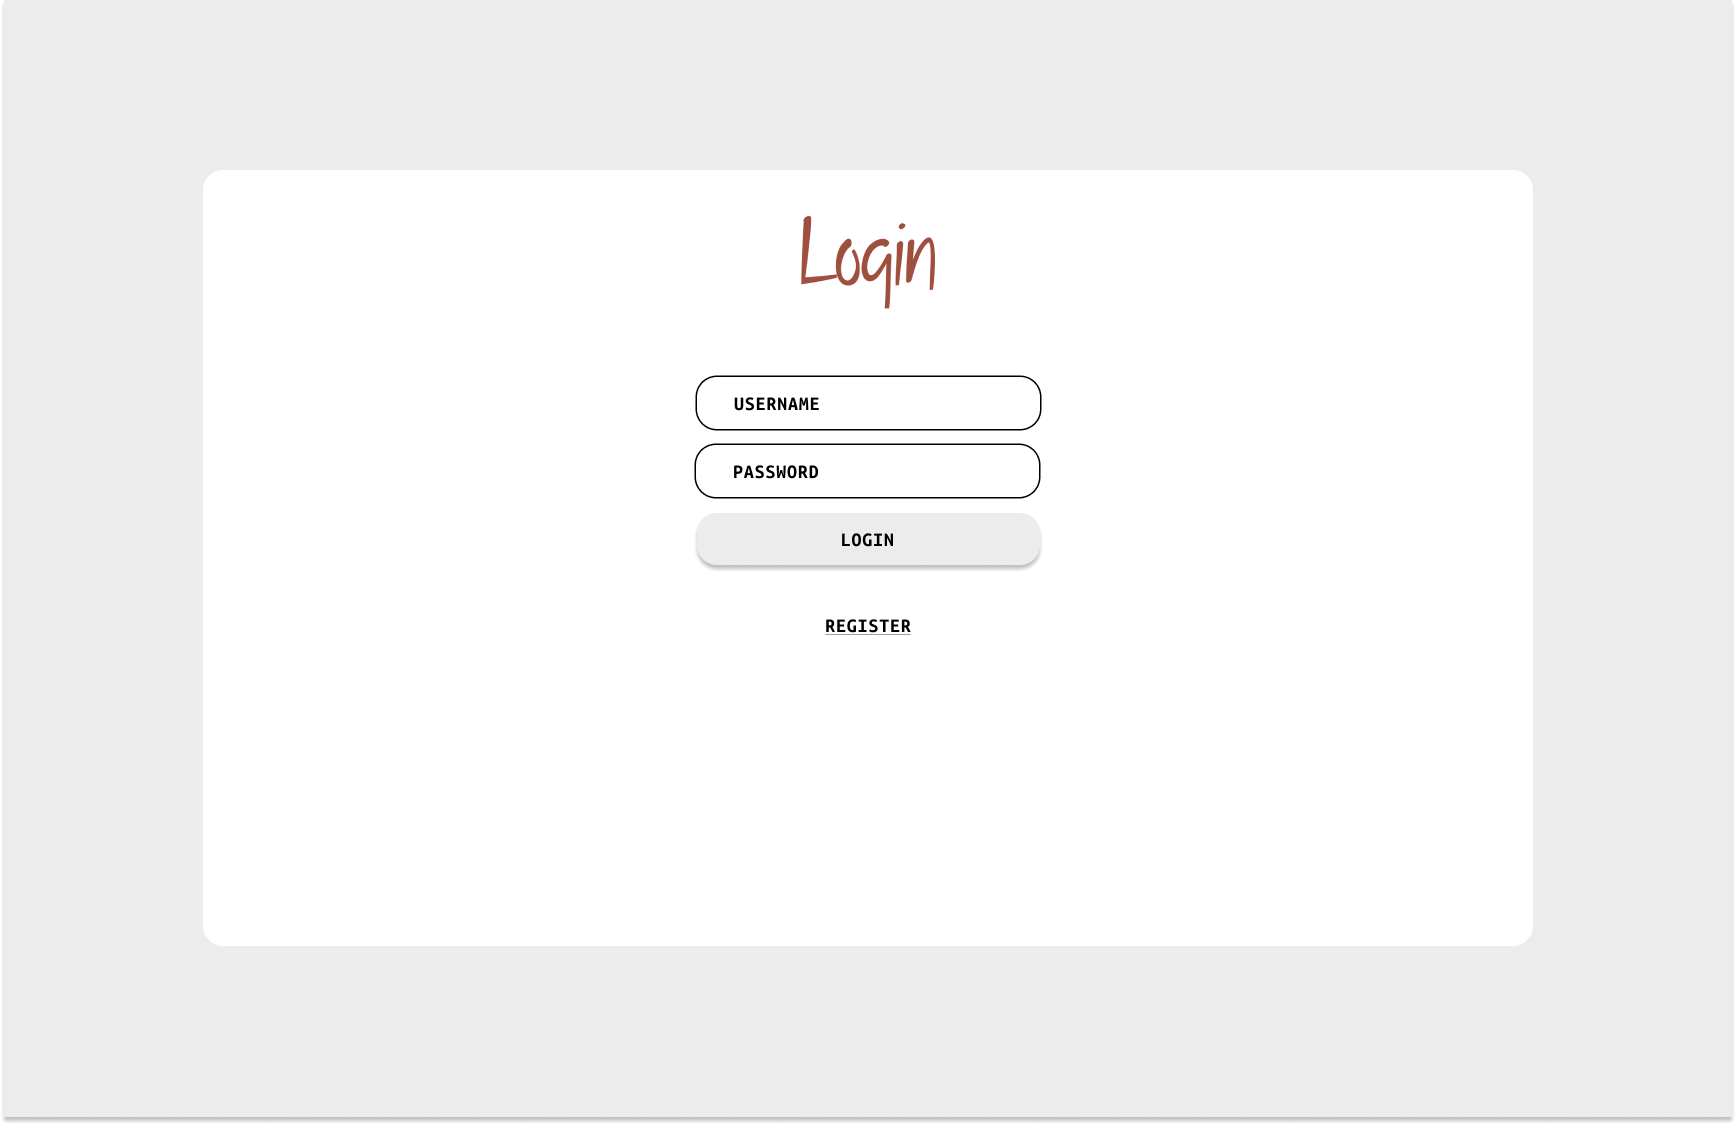
\includegraphics[width=\linewidth]{Login Page Desktop Lightfigma-mockups.png}
    \caption{Mockup für Login-Page auf Desktop im Light-Mode}
    \label{fig:Login Page Desktop Light}
\end{figure}

Auf der Overview-Page werden dem Nutzer empfohlende Artikel und Feeds vorgeschlagen. Dabei kann in eine detailierte Sicht für den Artikel gewechselt werden mit einem Klick auf einen Artikel. (vgl. Abbildung~\ref{fig:Overview Page Desktop Light})

\begin{figure}[H]
    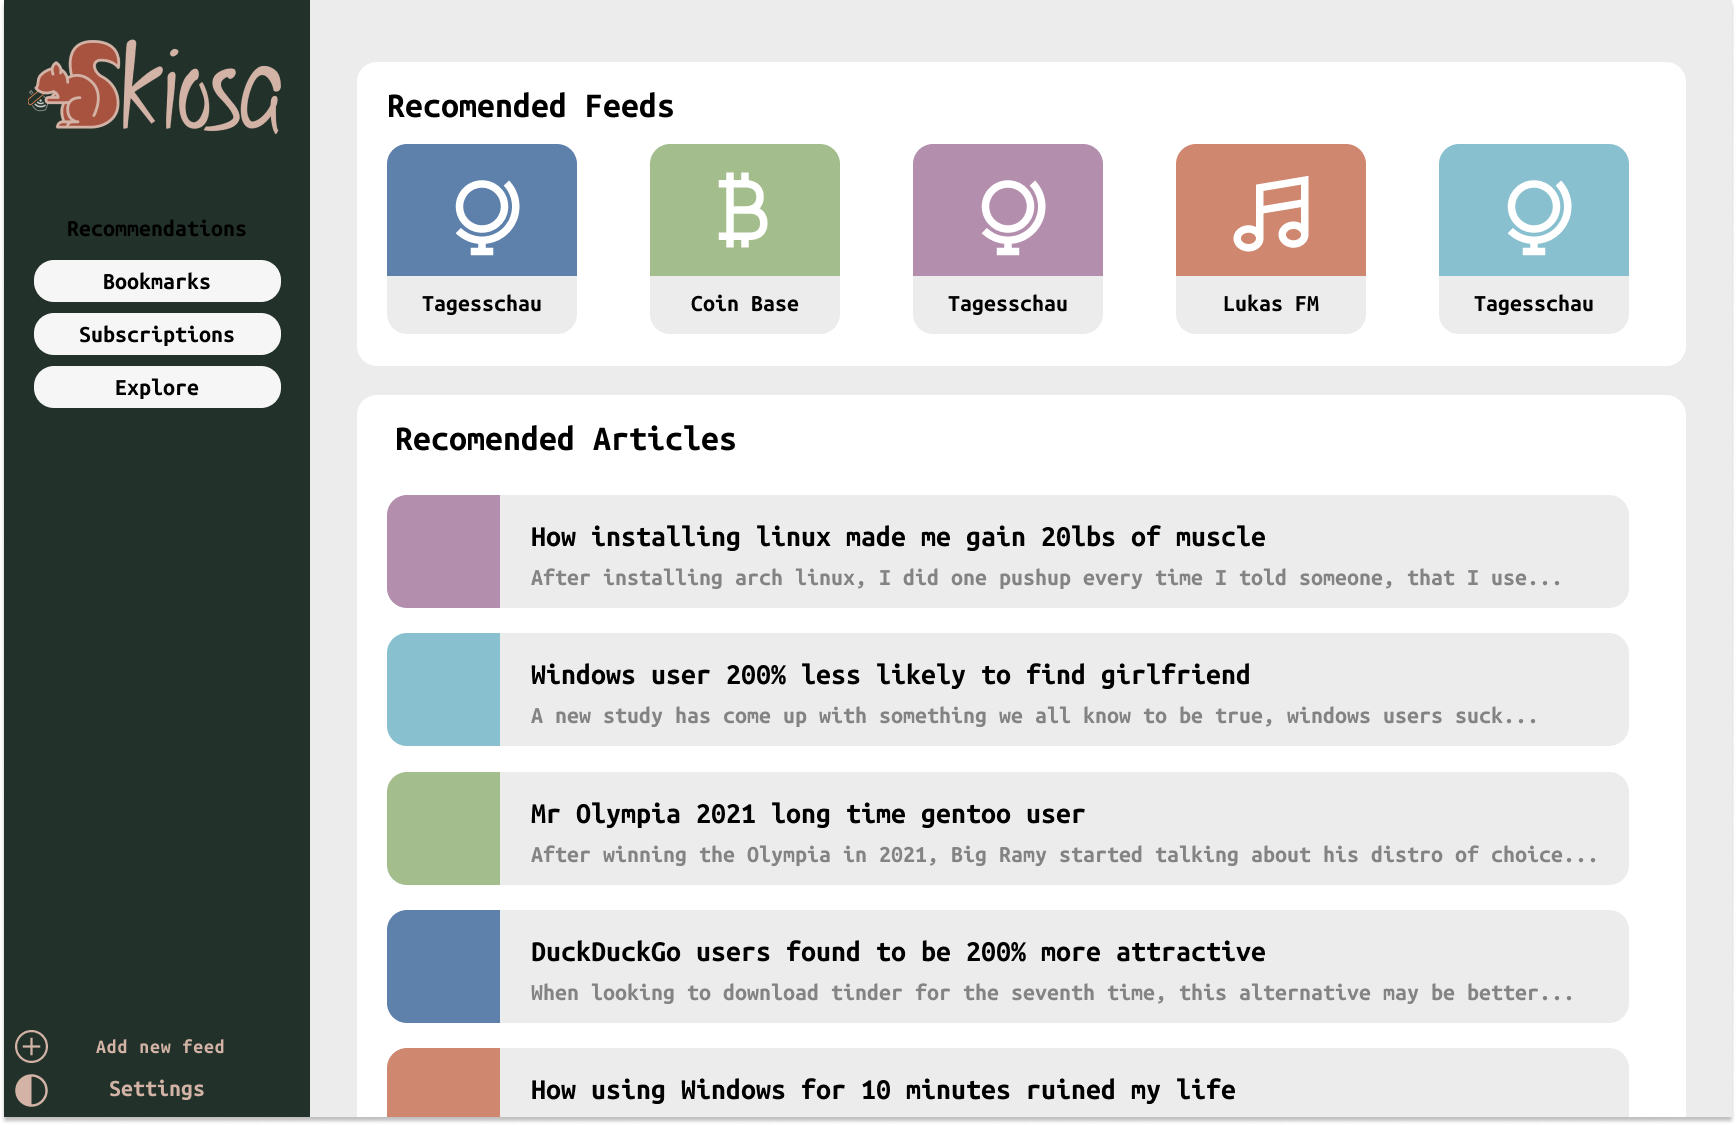
\includegraphics[width=\linewidth]{Overview Page Desktop Lightfigma-mockups.png}
    \caption{Mockup für Overview-Page auf Desktop im Light-Mode}
    \label{fig:Overview Page Desktop Light}
\end{figure}

In den Einstellungen hat der Nutzer die Möglichkeit seine Konto-Einstellungen anzupassen oder zwischen dem Light- und Darkmodus zu wechseln. (vgl. Abbildung~\ref{fig:Settings Interface Desktop Light})

\begin{figure}[H]
    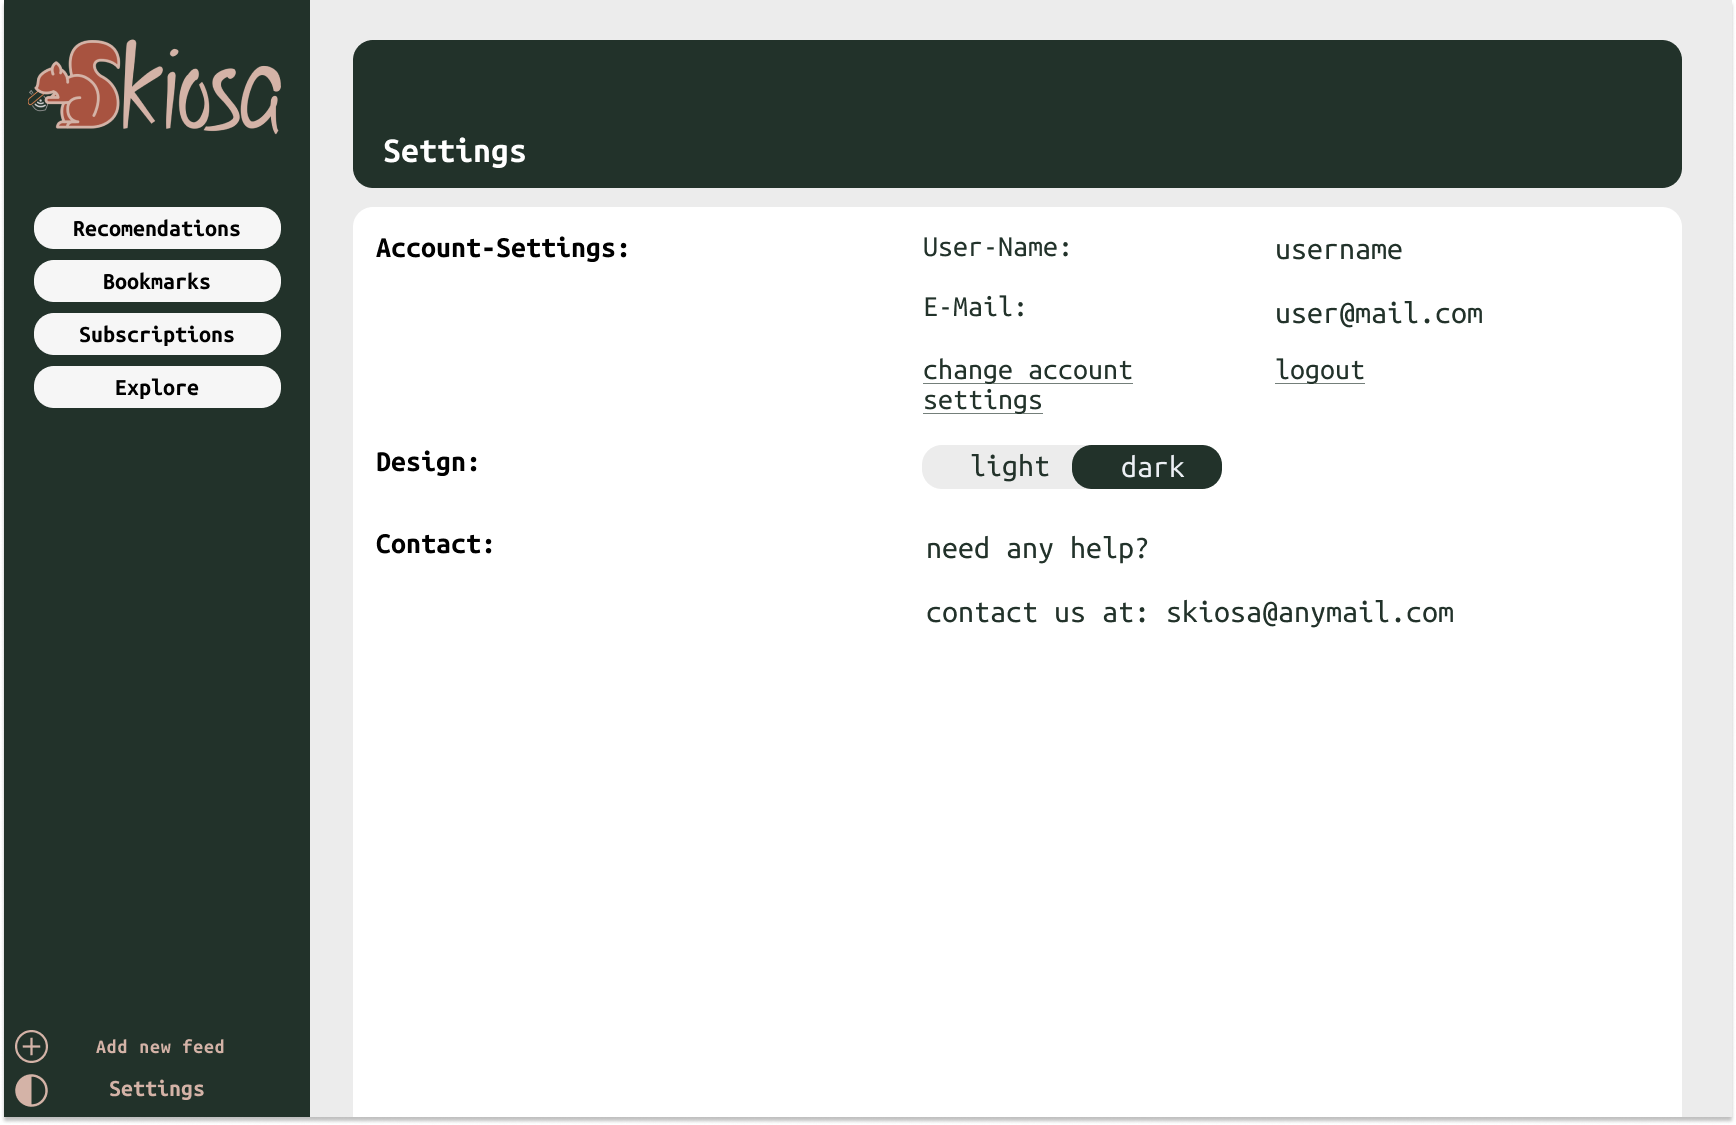
\includegraphics[width=\linewidth]{images/Settings Interface Desktop Lightfigma-mockups.png}
    \caption{Mockup für Settingspage auf Desktop im Light-Mode}
    \label{fig:Settings Interface Desktop Light}
\end{figure}

Auf der Subscription-Page werden alle abbonierten RSS-Feeds angezeigt. Dabei können mit einem Klick auf den Pfeil auf der rechten Seite die letzten veröffentlichten Artikel dieses Feeds angezeigt werden. (vgl. Abbildung~\ref{fig:Subscription Interface Desktop Light})

\begin{figure}[H]
    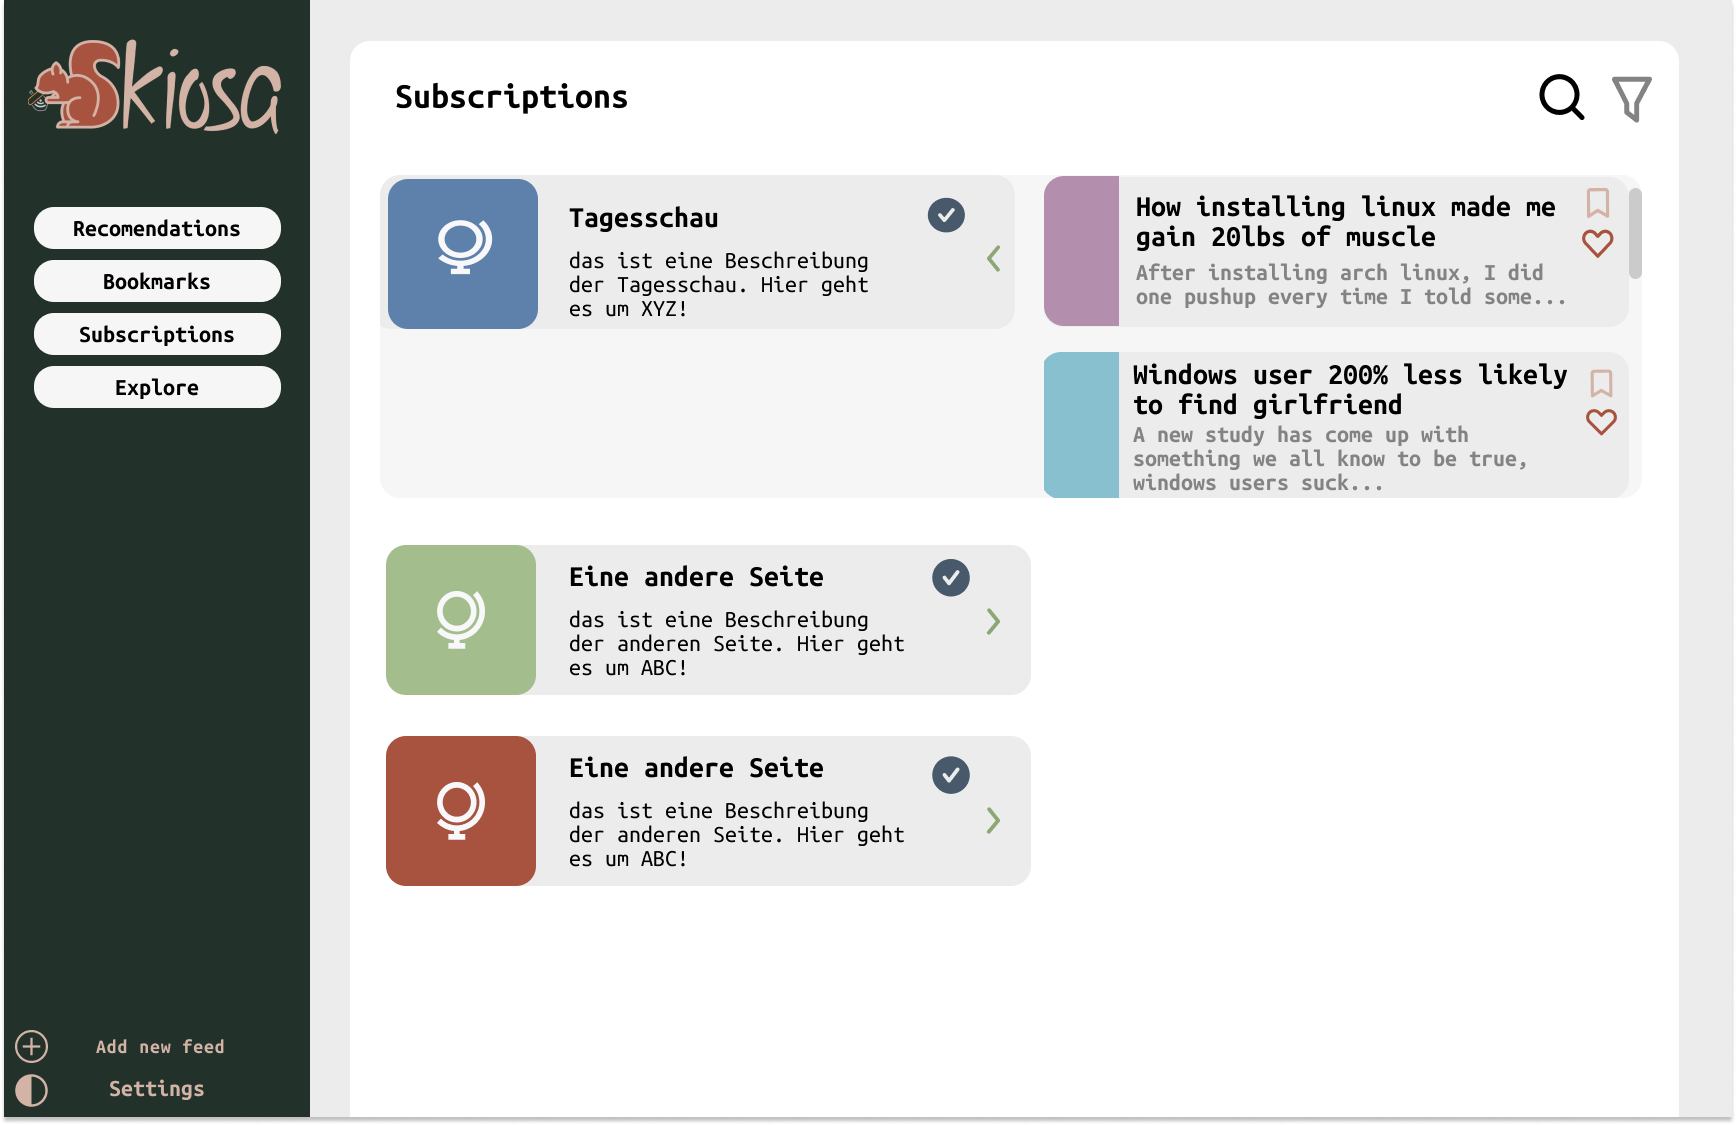
\includegraphics[width=\linewidth]{images/Subscription Interface Desktop Lightfigma-mockups.png}
    \caption{Mockup für Subscription-Page auf Desktop im Light-Mode}
    \label{fig:Subscription Interface Desktop Light}
\end{figure}

Auf der Article-View-Page werden die Details des Artikel angezeigt. Dabei kann man den Link zu dem Artikes teilen, den Artikel liken und bookmarken. 
Darüber hinaus gibt es Links zum Originalartikel und zum Feed, indem der Artikel veröffentlicht wurde. Unter \enquote{Similar Articles} werden zum Artikel ähnliche Artikel angezeigt. (vgl. Abbildung~\ref{fig:View Page Desktop Light})

\begin{figure}[H]
    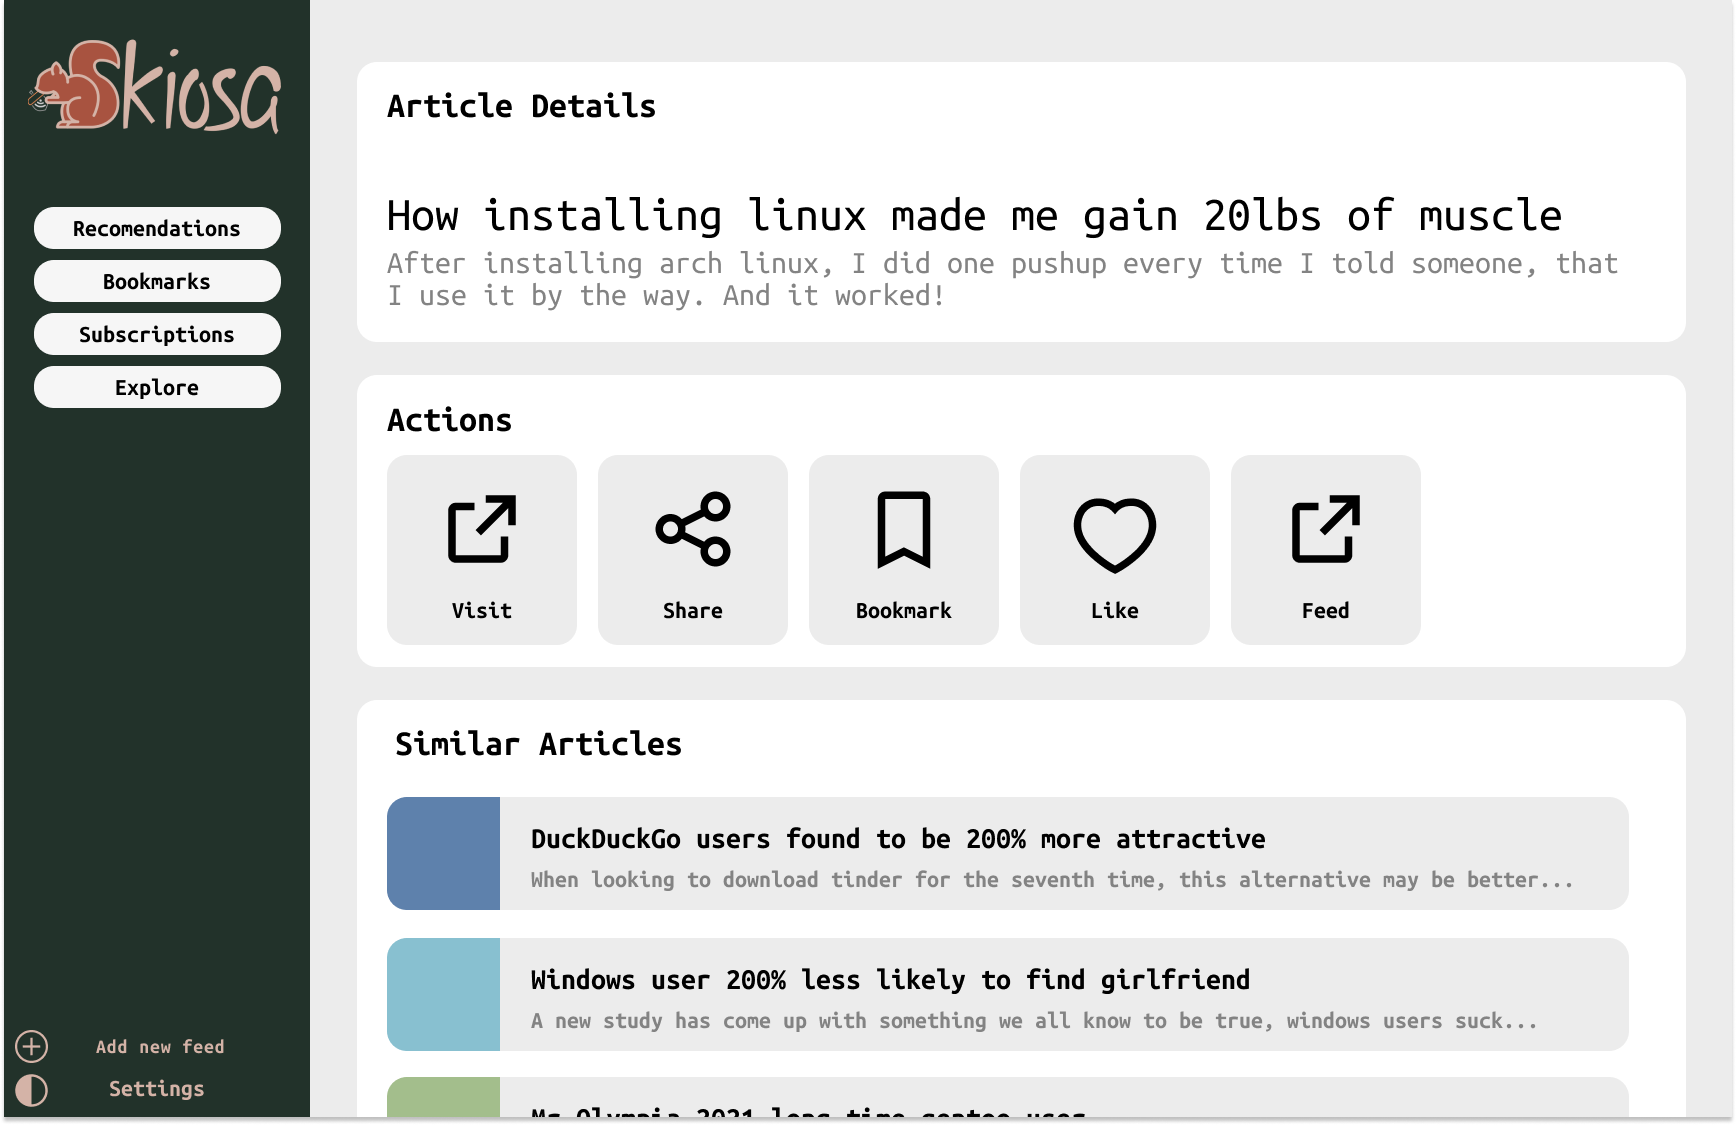
\includegraphics[width=\linewidth]{images/View Page Desktop Lightfigma-mockups.png}
    \caption{Mockup für Article-View-Page auf Desktop im Light-Mode}
    \label{fig:View Page Desktop Light}
\end{figure}

Für jede Page wurde dabei ein Mockup für den Light-Mode, 
für den Dark-Mode in der Desktop-Ansicht und ein Mockup im 
Light-Mode und ein Mockup im Dark-Mode in der mobilen Ansicht 
erstellt. Zur Feed-Overview-Page sehen diese folgendermaßen aus:

\begin{figure}[H]
    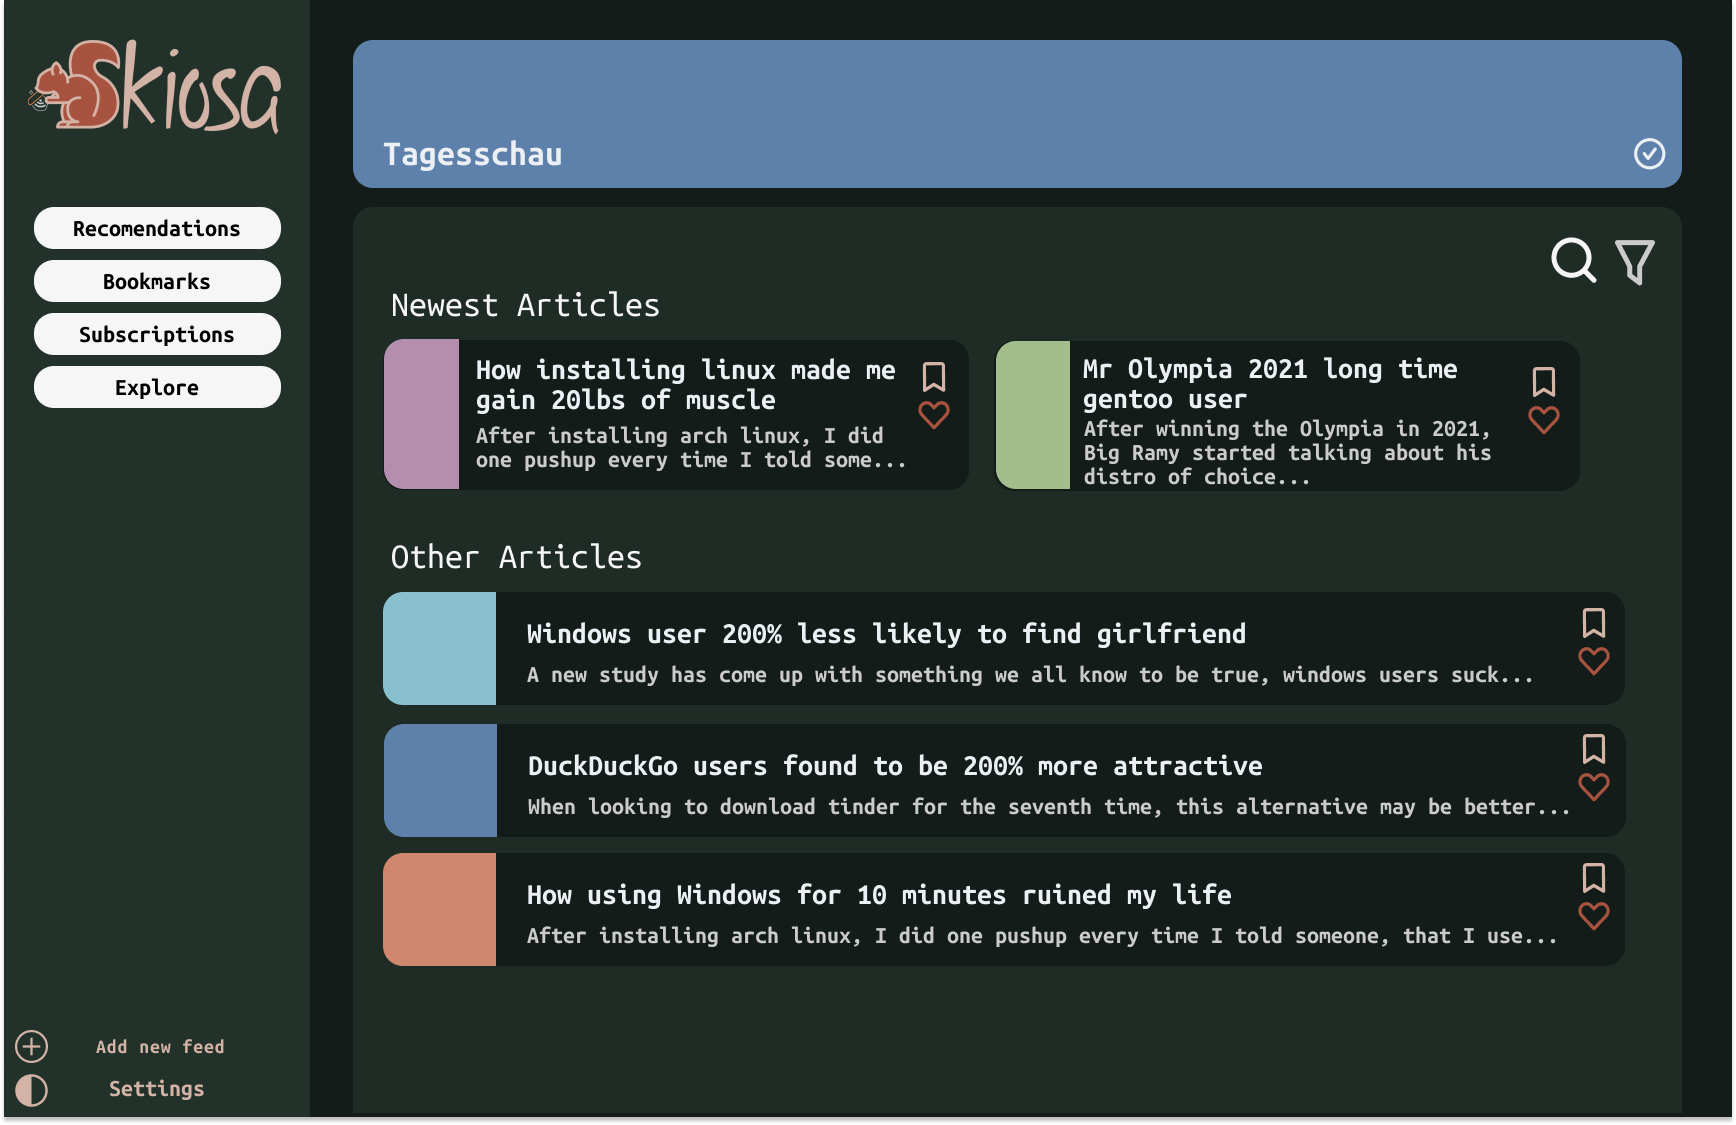
\includegraphics[width=\linewidth]{Feed Overview Page Desktop Darkfigma-mockups.png}
    \caption{Mockup für Feed-Overview-Page auf Desktop im Dark-Mode}
    \label{fig:Feed Overview Page Dark Desktop}
\end{figure}

\begin{figure}[H]
    \begin{center}
        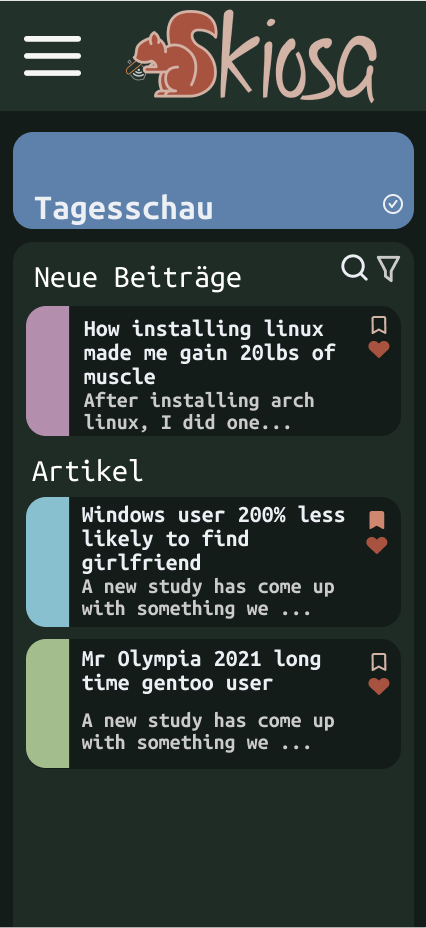
\includegraphics[height=10cm]{Feed Overview Page Mobile Darkfigma-mockups.png}
    \end{center}
    \caption{Mockup für Feed-Overview-Page auf Mobile im Dark-Mode}
    \label{fig:Feed Overview Page Light Mobile}
\end{figure}


\begin{figure}[H]
    \begin{center}
        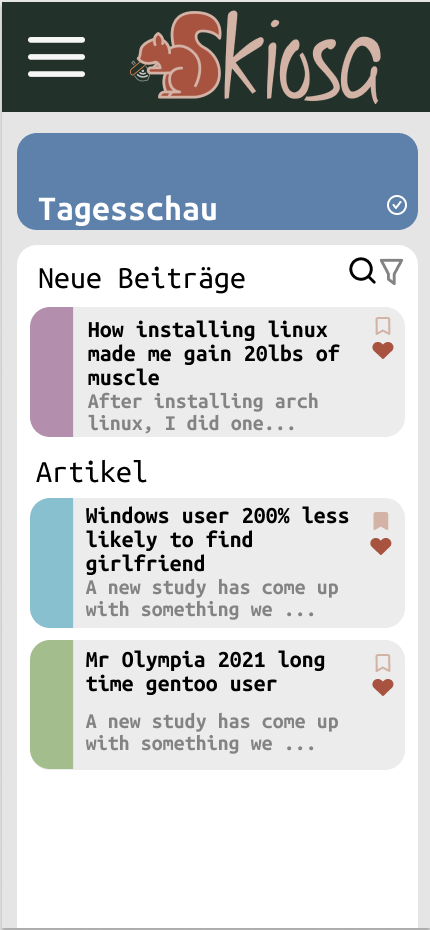
\includegraphics[height=10cm]{Feed Overview Page Mobile Lightfigma-mockups.png}
    \end{center}
    \caption{Mockup für Feed-Overview-Page auf Mobile im Light-Mode}
    \label{fig:Feed Overview Page Light Mobile}
\end{figure}


\subsection{Erläuterung zur Funktionalität einzelner Seiten}

Um zusätzliche Fragen, wie etwa die Funktionalität einzelner Mockups und unserer Plattform zu erklären, wurden nachtäglich ebenfalls Aktivitätsdiagramme zu den einzelnen Seiten (bzw. globalen Komponenten) erstellt.
Diese erläutern das Verhalten verschiedener Seiten und werden im Folgenden erläutert.

Das Aktivitätsdiagram der Loginseite ist in Abbildung~\ref{fig:umlActivityLogin.png} dargestellt.
Auf dieser Seite ist es möglich kann man sich entweder direkt mit Username und Passwort anmelden oder auf registrieren klicken.
Sind die Anmeldedaten korrekt wird man eingeloggt, sind die Anmeldedaten fehlerhaft können diese korrigiert werden.
\begin{figure}
    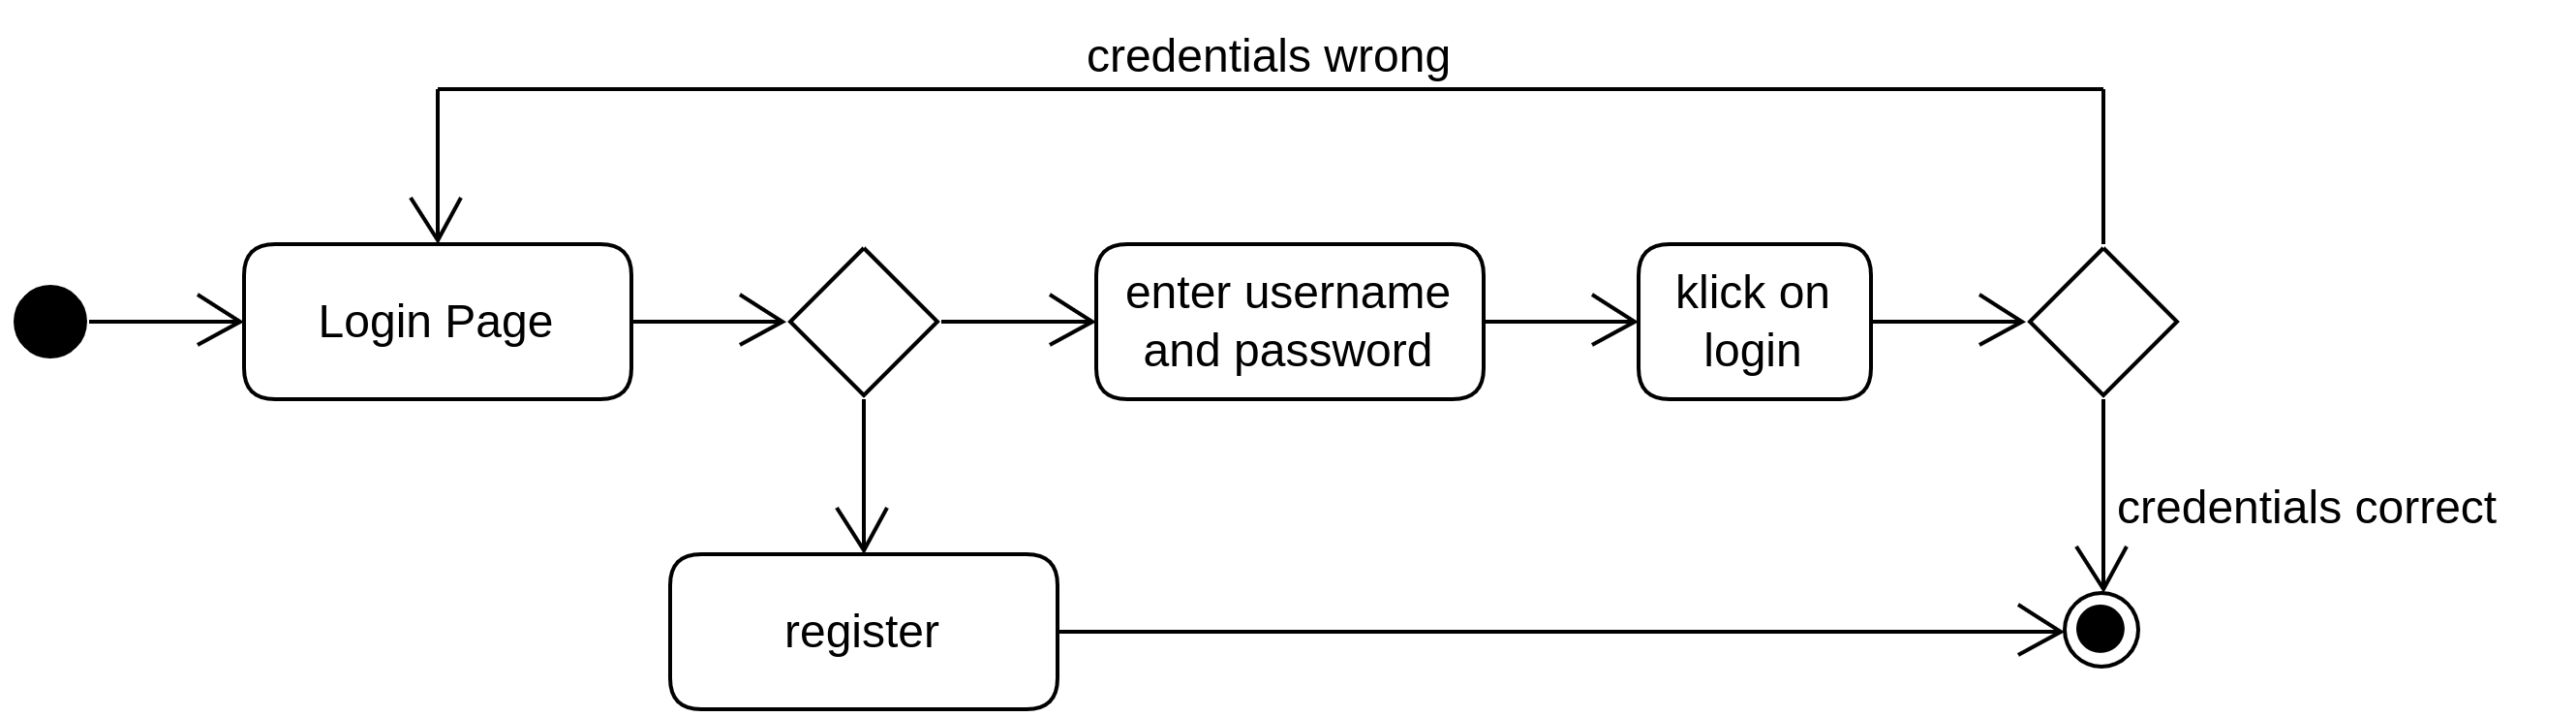
\includegraphics[width=\linewidth]{umlActivityLogin.png}
    \caption{Aktivitätsdiagramm der Loginseite}
    \label{fig:umlActivityLogin.png}
\end{figure}

In Abbildung~\ref{fig:umlActivityRegister.png} wird die Registrierungsseite beschrieben.
Auf der Seite müssen Daten, wie Vorname, Nachname, E-Mail, Benutzername, sowie Passwort und dessen Wiederholung eingetragen werden.
Sind die Registrierungsdaten korrekt, bzw. nicht bereits registriert (z.B. Benutzername) kann mit Bestätigung auf registrieren ein User angelegt werden.
Zu jedem Zeitpunkt kann die Registrierung abgebrochen und zur Loginseite zurückgekehrt werden.
\begin{figure}
    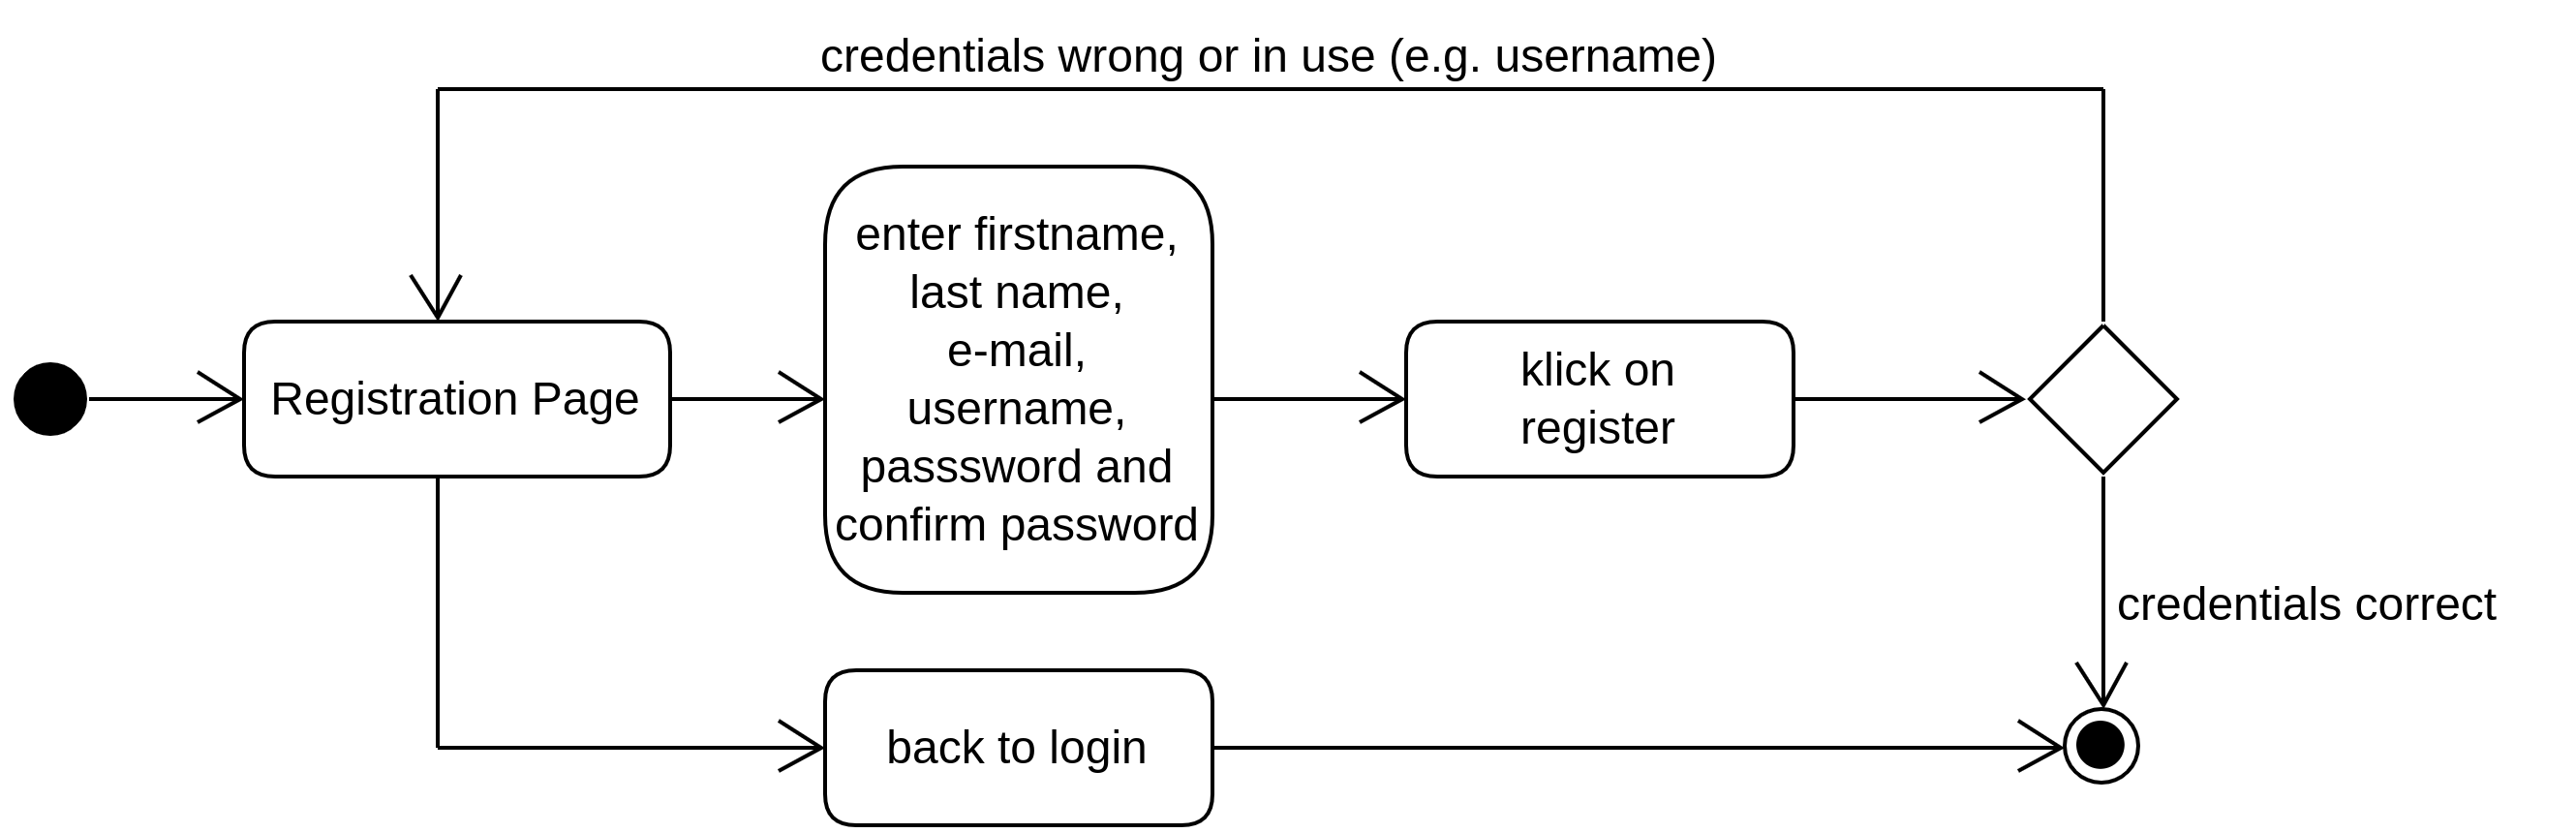
\includegraphics[width=\linewidth]{umlActivityRegister.png}
    \caption{Aktivitätsdiagramm der Registrierungsseite}
    \label{fig:umlActivityRegister.png}
\end{figure}

Die Seitenleiste ist auf jeder Seite mit Außnahme Login- und Registrierungsseite, sowie während des Pop-ups zum Hinzufügen eines Feeds erreichbar.
In Abbildung~\ref{fig:umlActivitySidebar.png} werden die möglichen Aktionen der Seitenleiste dargestellt.
Von dieser kann direkt zwischen Dark- und Light-Mode umgeschalten werden. Zudem kann man sich einloggen
oder falls bereits geschehen auf die Einstellungen gewechselt werden. Die Schaltfläche des Login wird nach erfolgreichem Login auf Settings geändert.
Es kann immer auf die Empfehlungen zugegriffen werden, sowohl als eingeloggter wie auch als nicht eingeloggter Nutzer.
Unter der Voraussetzung, dass der Benutzer eingeloggt ist, kann direkt zu den Lesezeichen und den Abonnements gewechselt werden.
Zusätzlich kann direkt ein neuer RSS Feed hinzugefügt werden.
\begin{figure}
    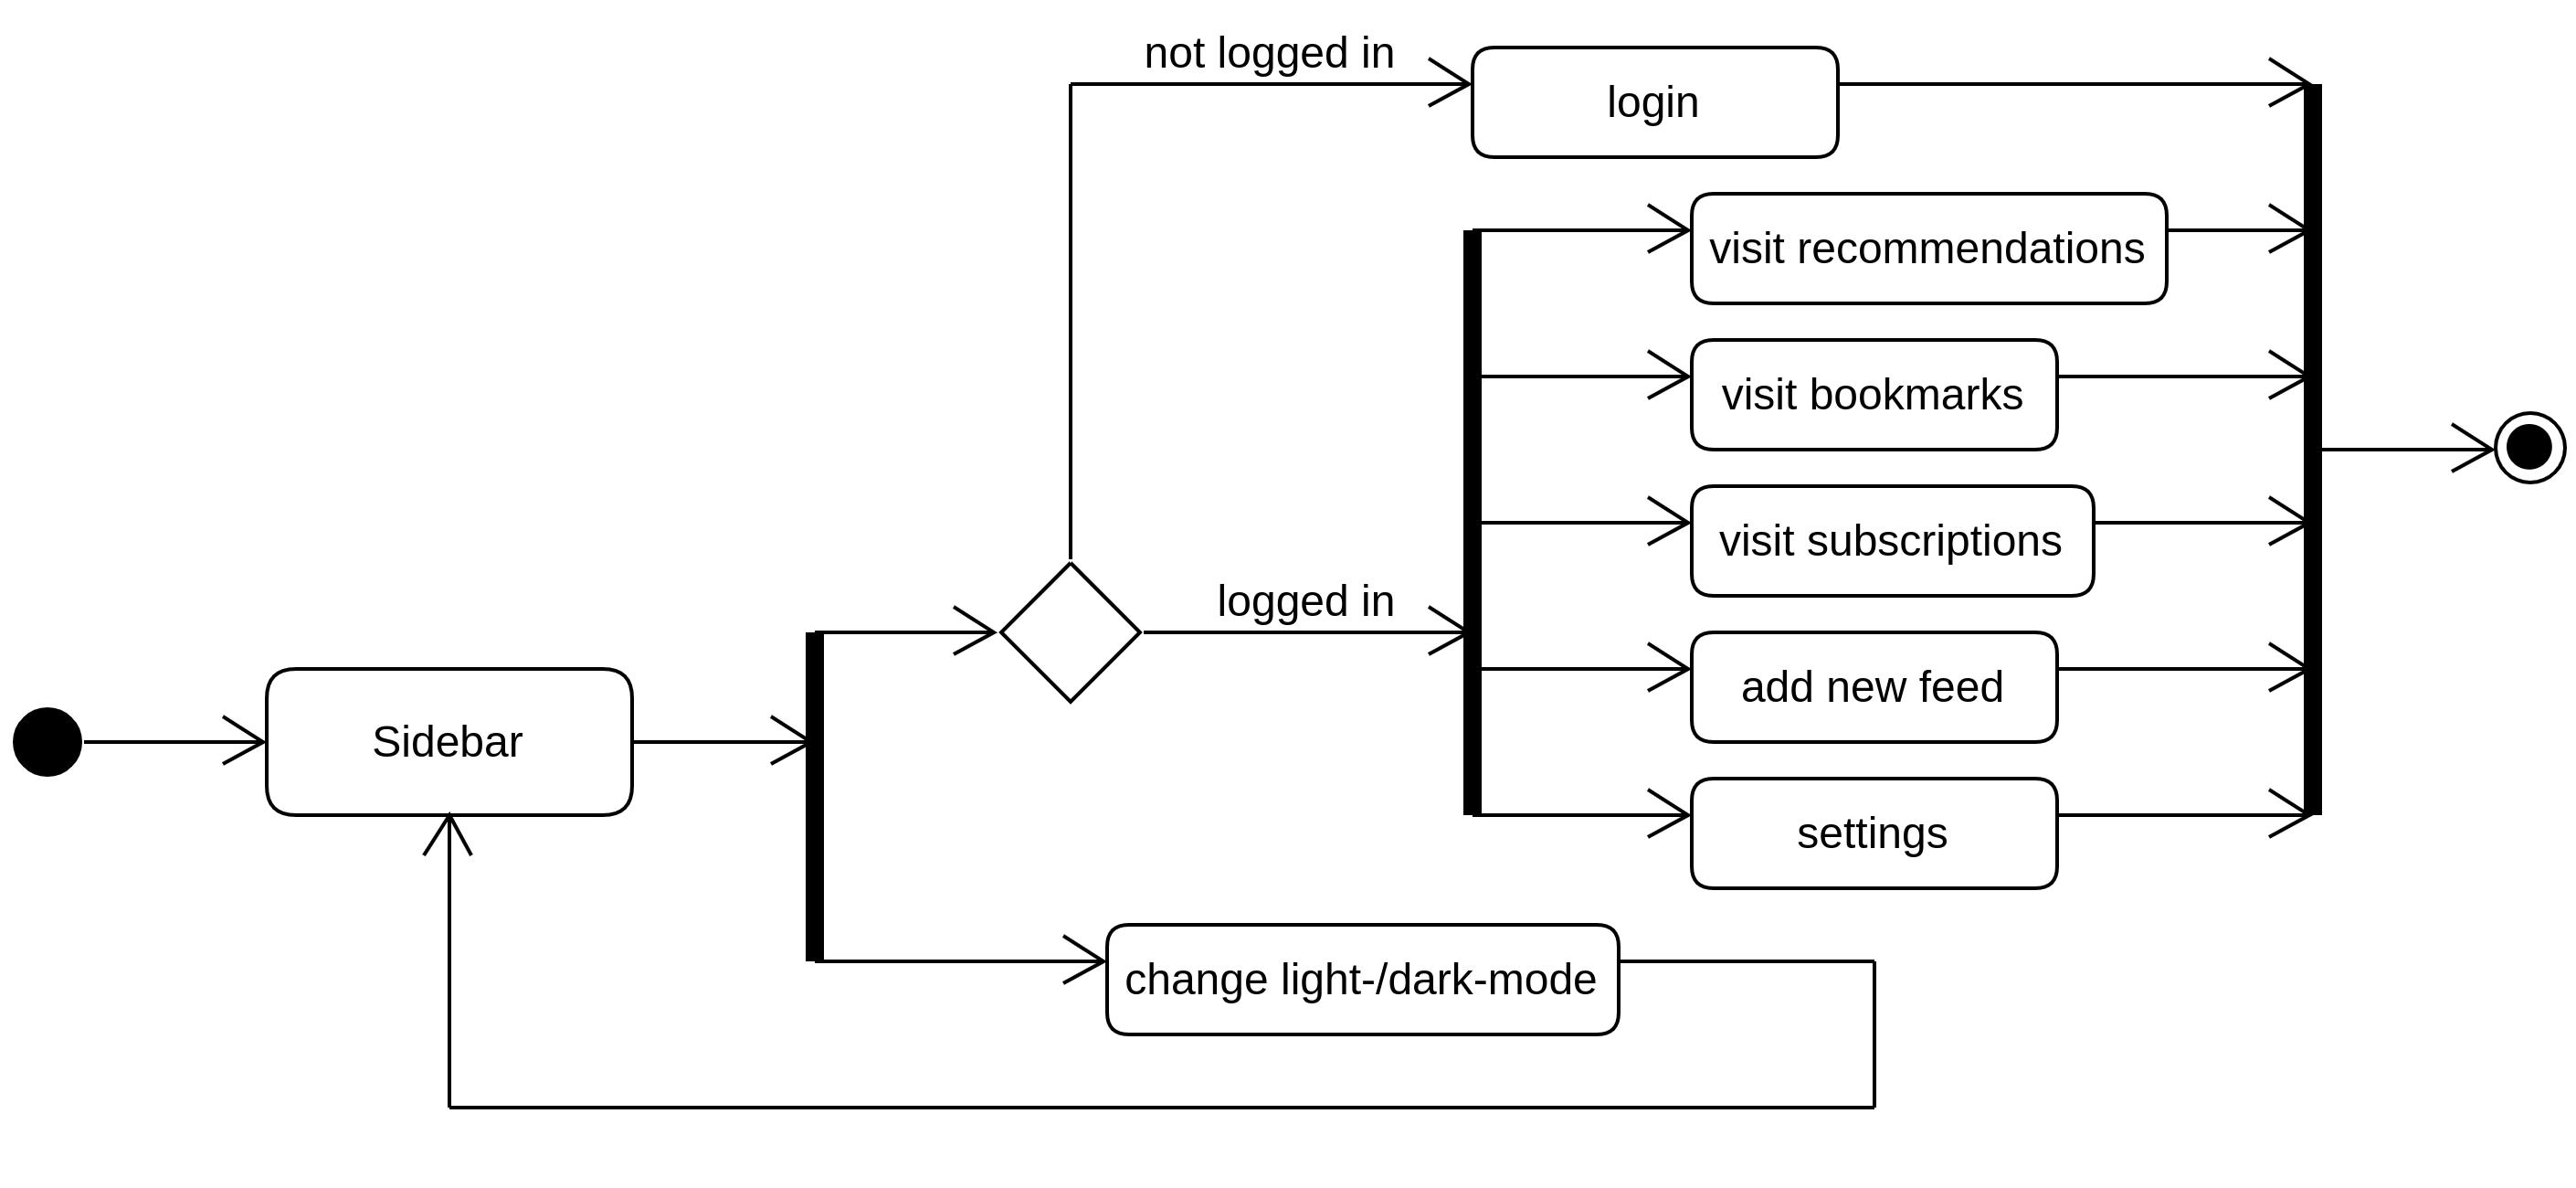
\includegraphics[width=\linewidth]{umlActivitySidebar.png}
    \caption{Aktivitätsdiagramm der Seitenleiste}
    \label{fig:umlActivitySidebar.png}
\end{figure}

Auf der Übersichtsseite können empfohlene Feeds oder empfohlene Artikel besucht werden.
Das Aktivitätsdiagramm ist in Abbildung~\ref{fig:umlActivityOverview.png} dargestellt.
\begin{figure}
    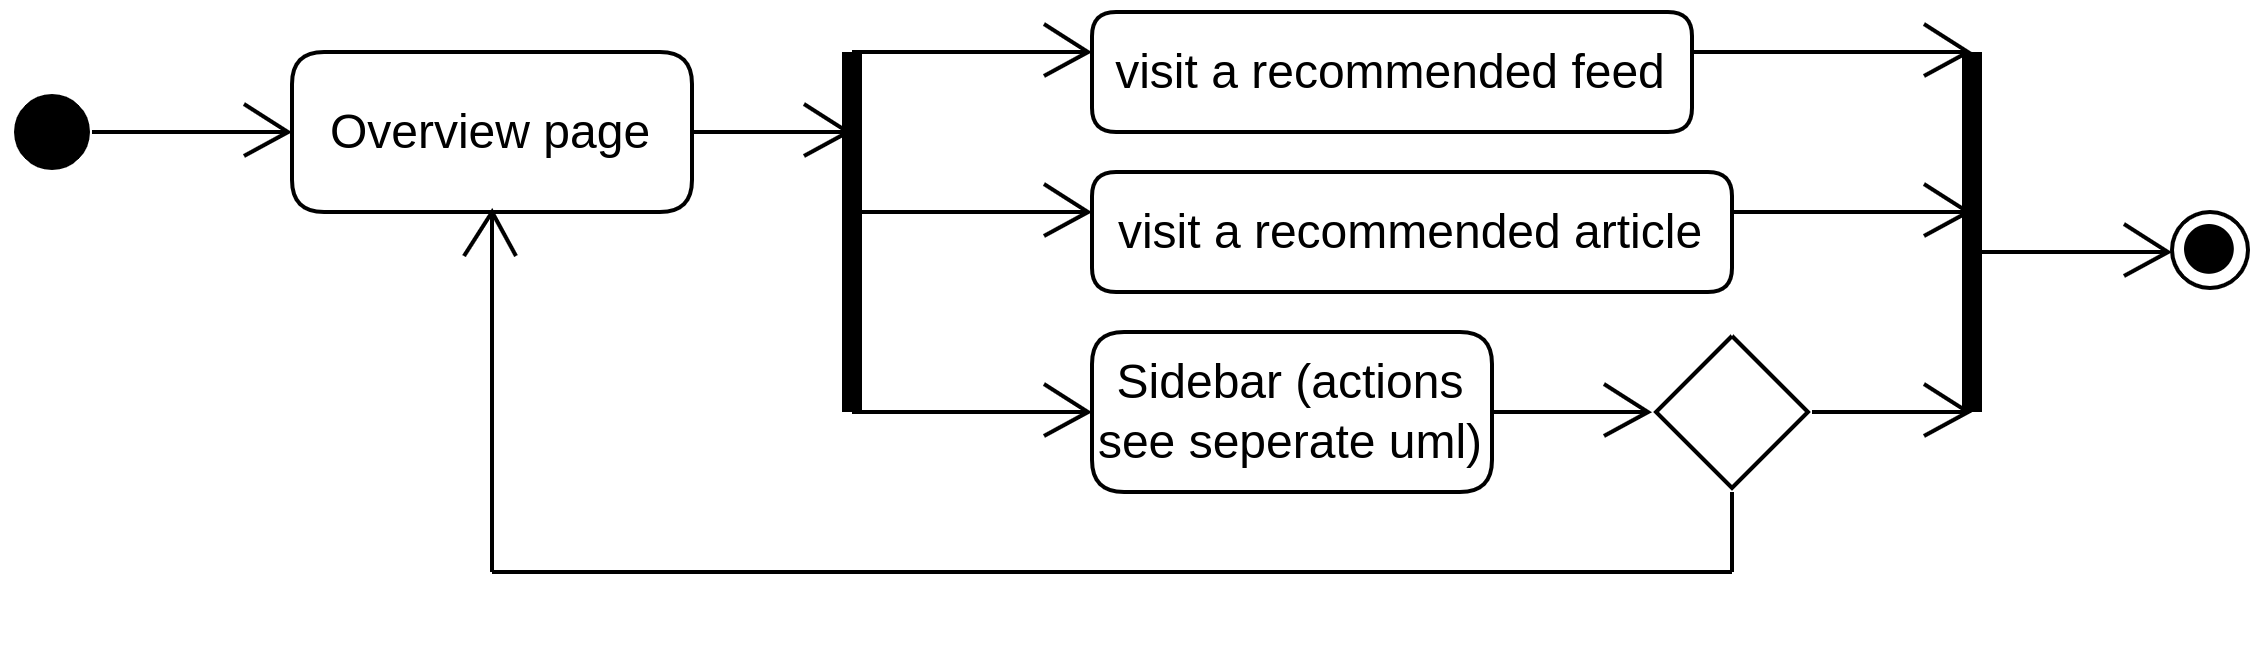
\includegraphics[width=\linewidth]{umlActivityOverview.png}
    \caption{Aktivitätsdiagramm der Übersichtsseite}
    \label{fig:umlActivityOverview.png}
\end{figure}

In Abbildung~\ref{fig:umlActivityFeed.png} werden die möglichen Aktionen auf der Feedseite dargestellt.
Der aufgerufene Feed kann abonniert und deabonniert werden. Im Feed kann gefiltert und/oder gesucht werden.
Einzelne Artikel können als Lesezeichen gespeichert oder geliked werden. Per Klick auf den Artikel kann dieser aufgerufen werden.
\begin{figure}
    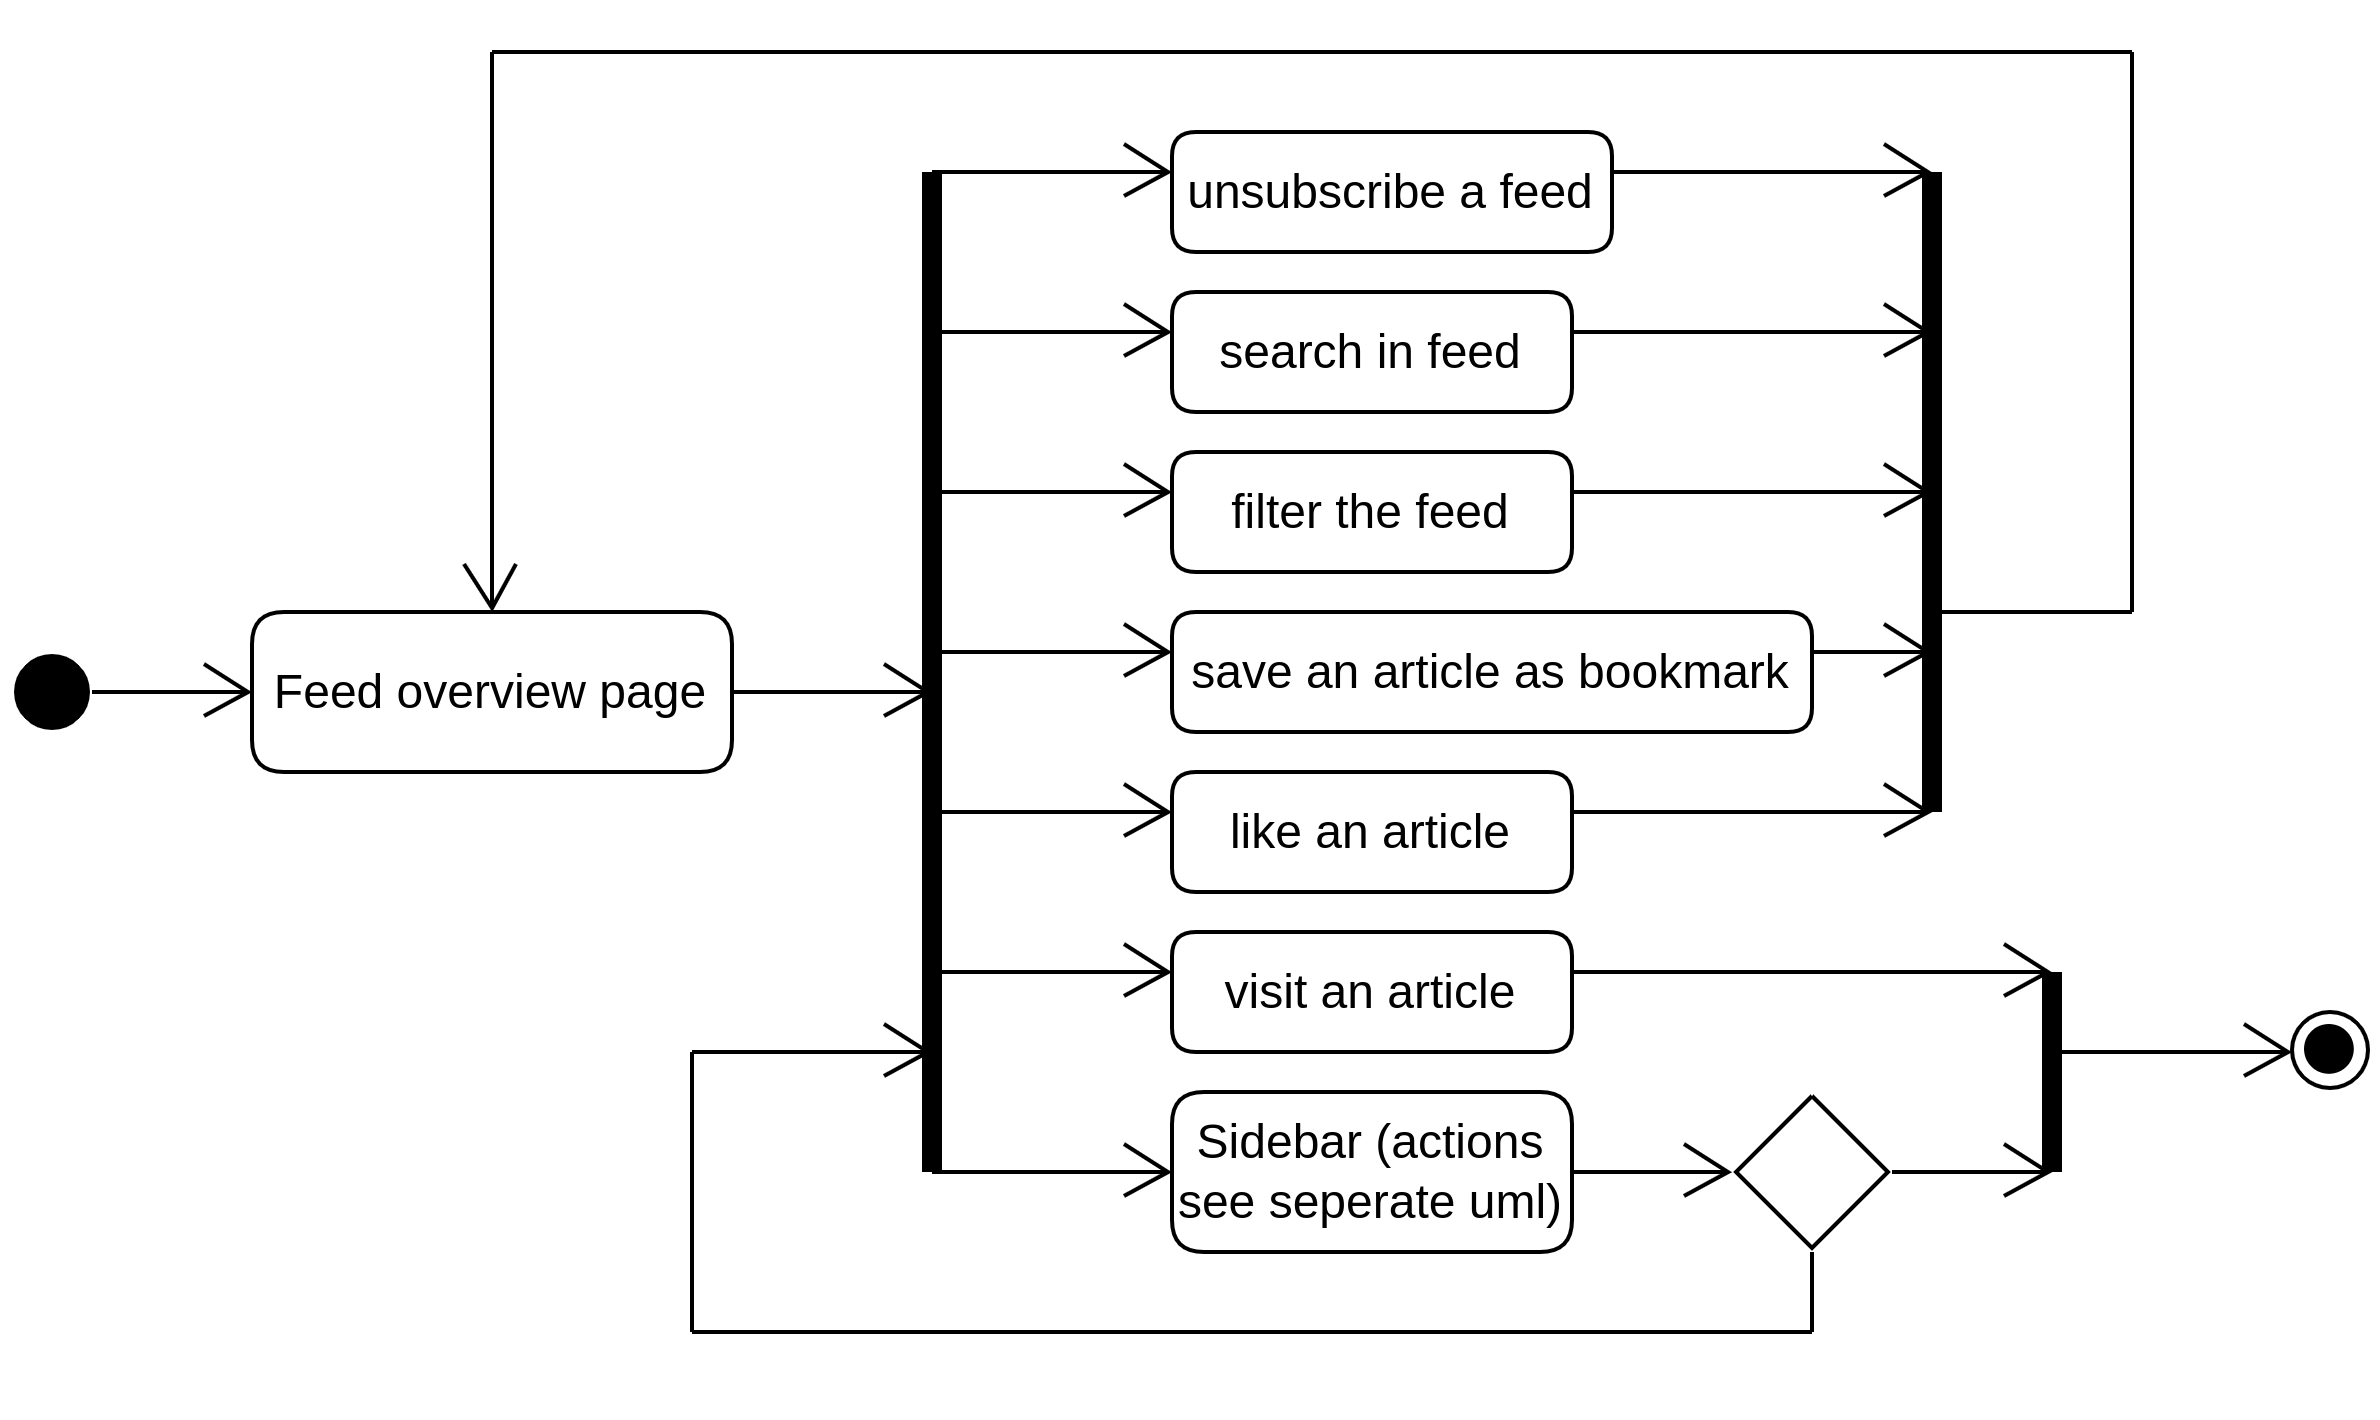
\includegraphics[width=\linewidth]{umlActivityFeed.png}
    \caption{Aktivitätsdiagramm der Feedseite}
    \label{fig:umlActivityFeed.png}
\end{figure}

Auf der Artikelseite kann, wie in Abbildung~\ref{fig:umlActivityView.png} dargestellt der Artikel gelesen werden.
Darüber hinaus kann der Artikel als Lesezeichen gespeichert, geliked und/oder geteilt werden (Link wird in die Zwischenablage kopiert).
Auch die Feedseite des Artikels kann aufgerufen werden. Die Ursprungswebseite des Artikels kann auch geöffnet werden.
Unter den ähnlichen Artikeln kann zu diesem per Klick gewechselt werden.
\begin{figure}
    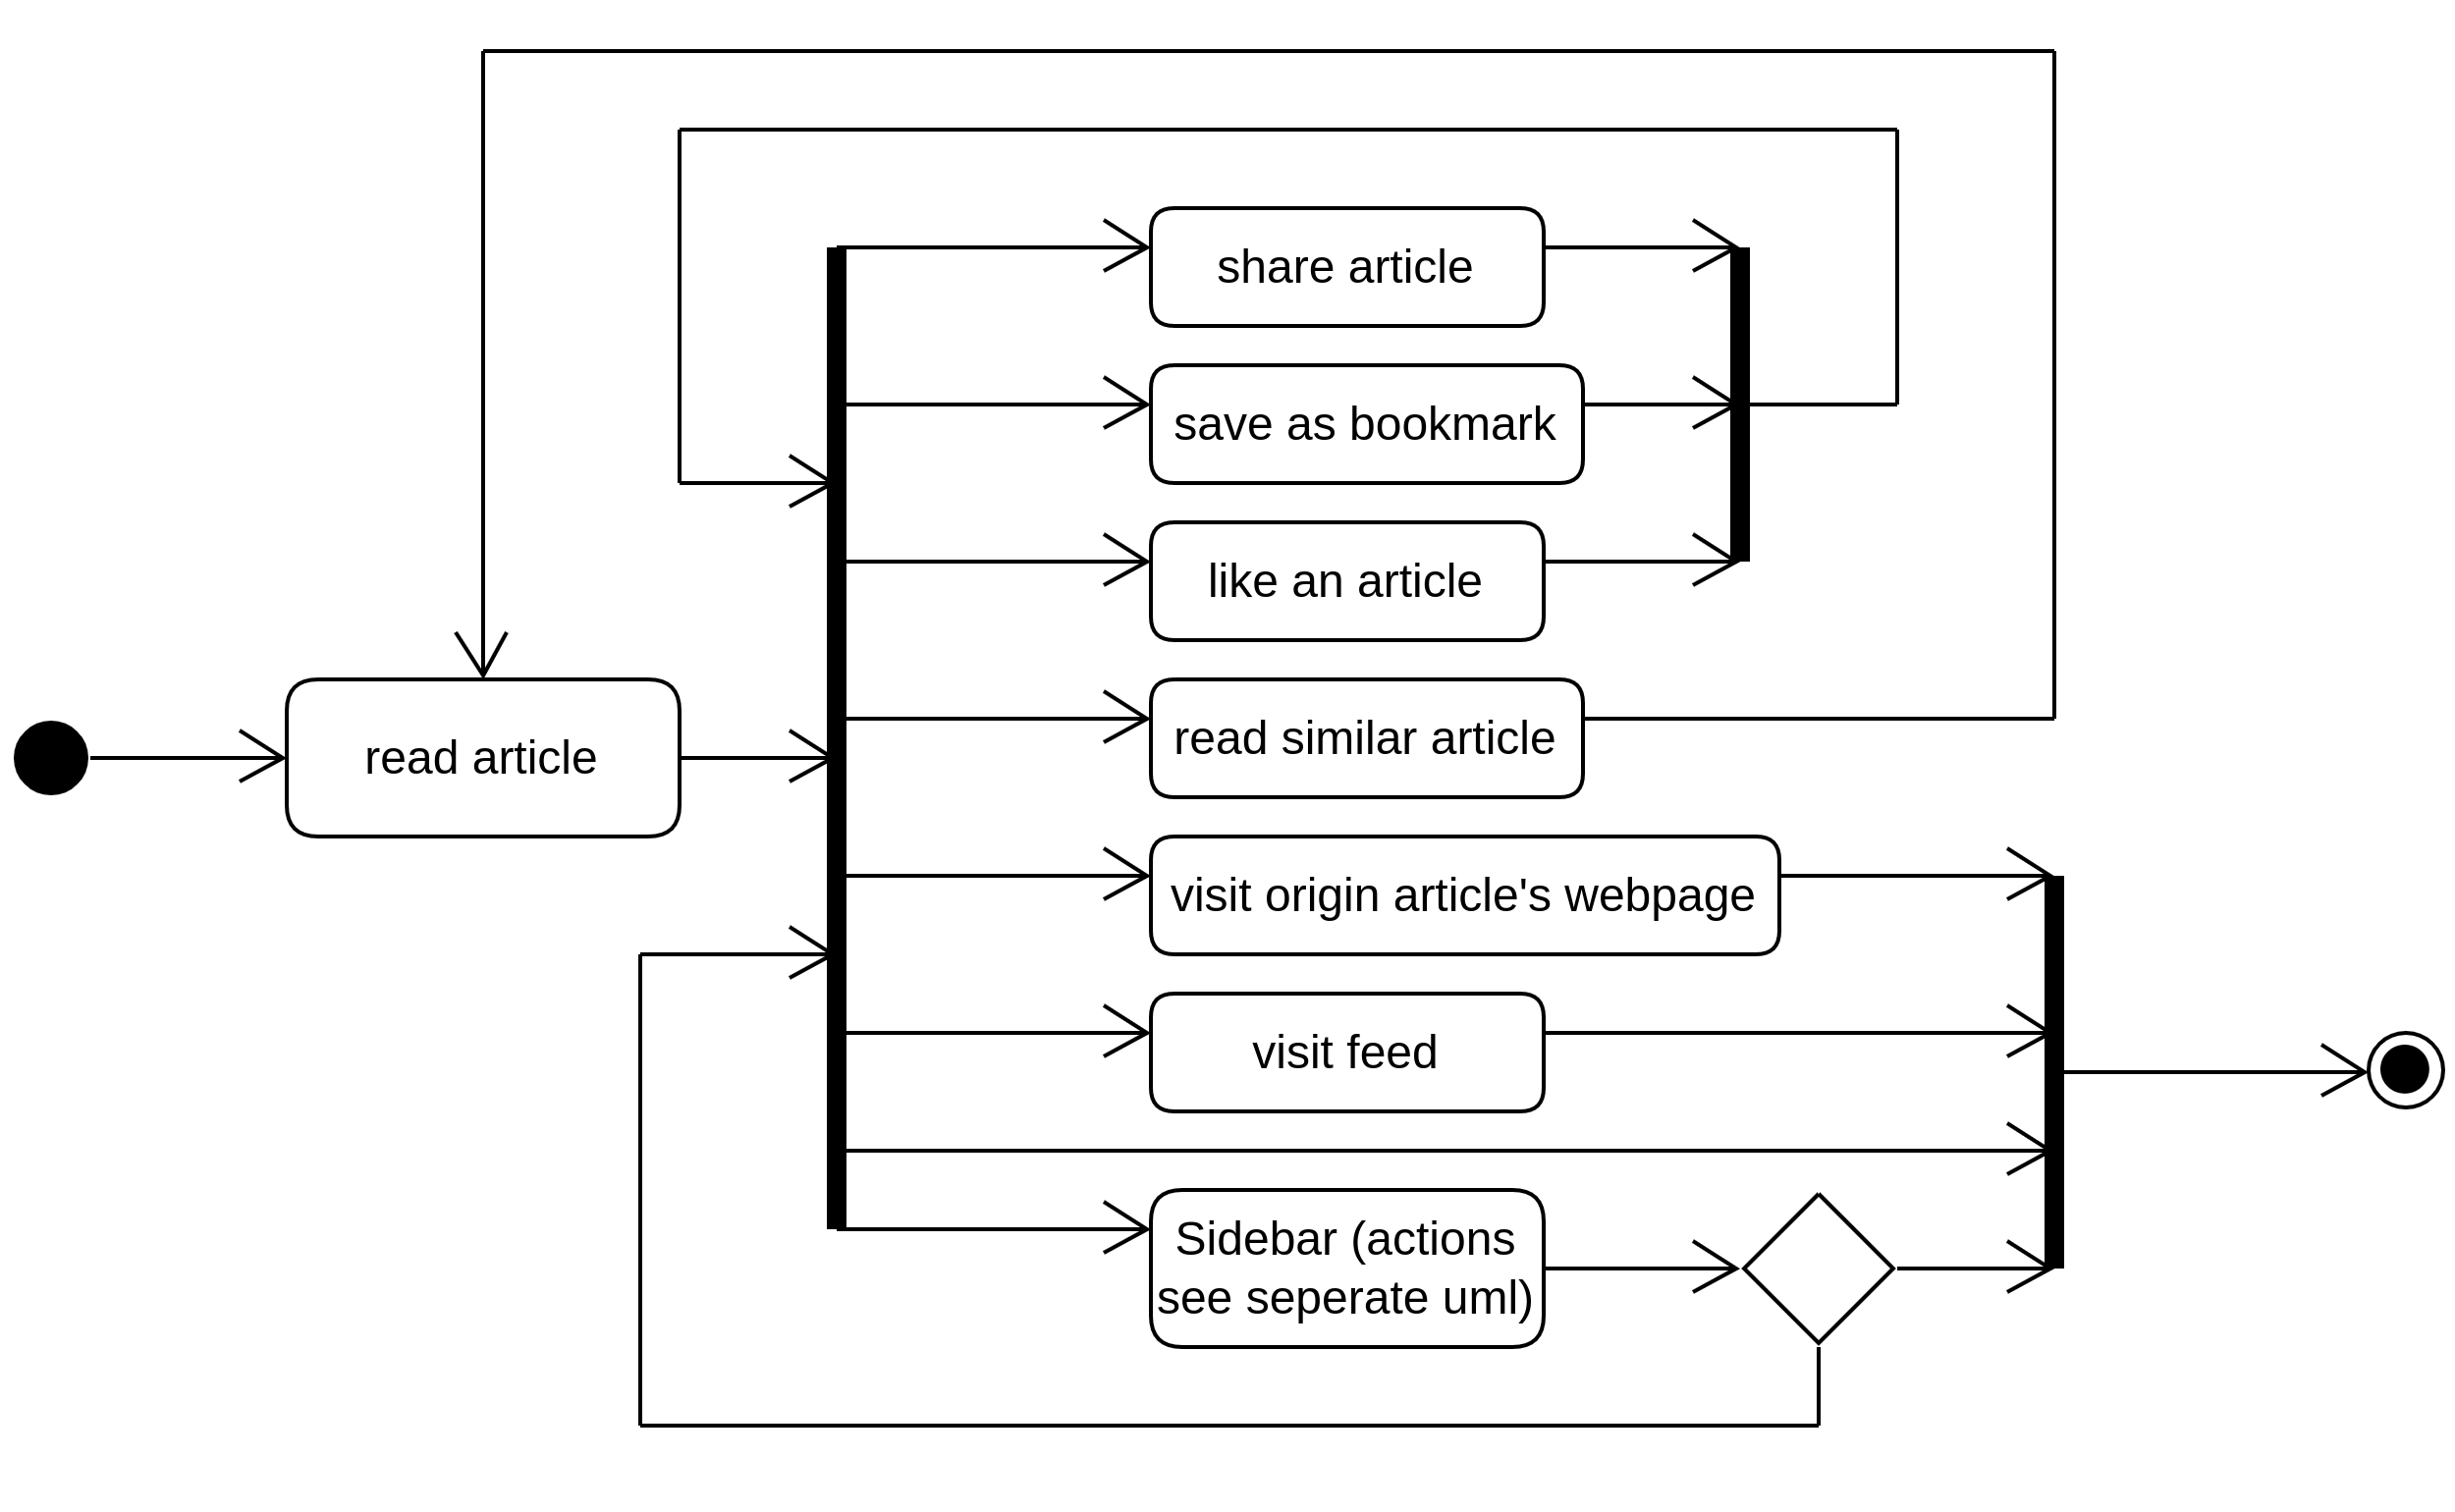
\includegraphics[width=\linewidth]{umlActivityView.png}
    \caption{Aktivitätsdiagramm der Artikelseite}
    \label{fig:umlActivityView.png}
\end{figure}


In Abbildung~\ref{fig:umlActivityBookmarks.png} ist das Aktivitätsdiagramm der Lesezeichenseite dargestellt.
Alle vom Nutzer gespeicherten Lesezeichen werden hier aufgelistet und es kann gefiltert und/ oder darin gesucht werden.
Einzelne Artikel können aus den Lesezeichen gelöscht werden. Auch können einzelne Artikel geliked oder entliked werden.
\begin{figure}
    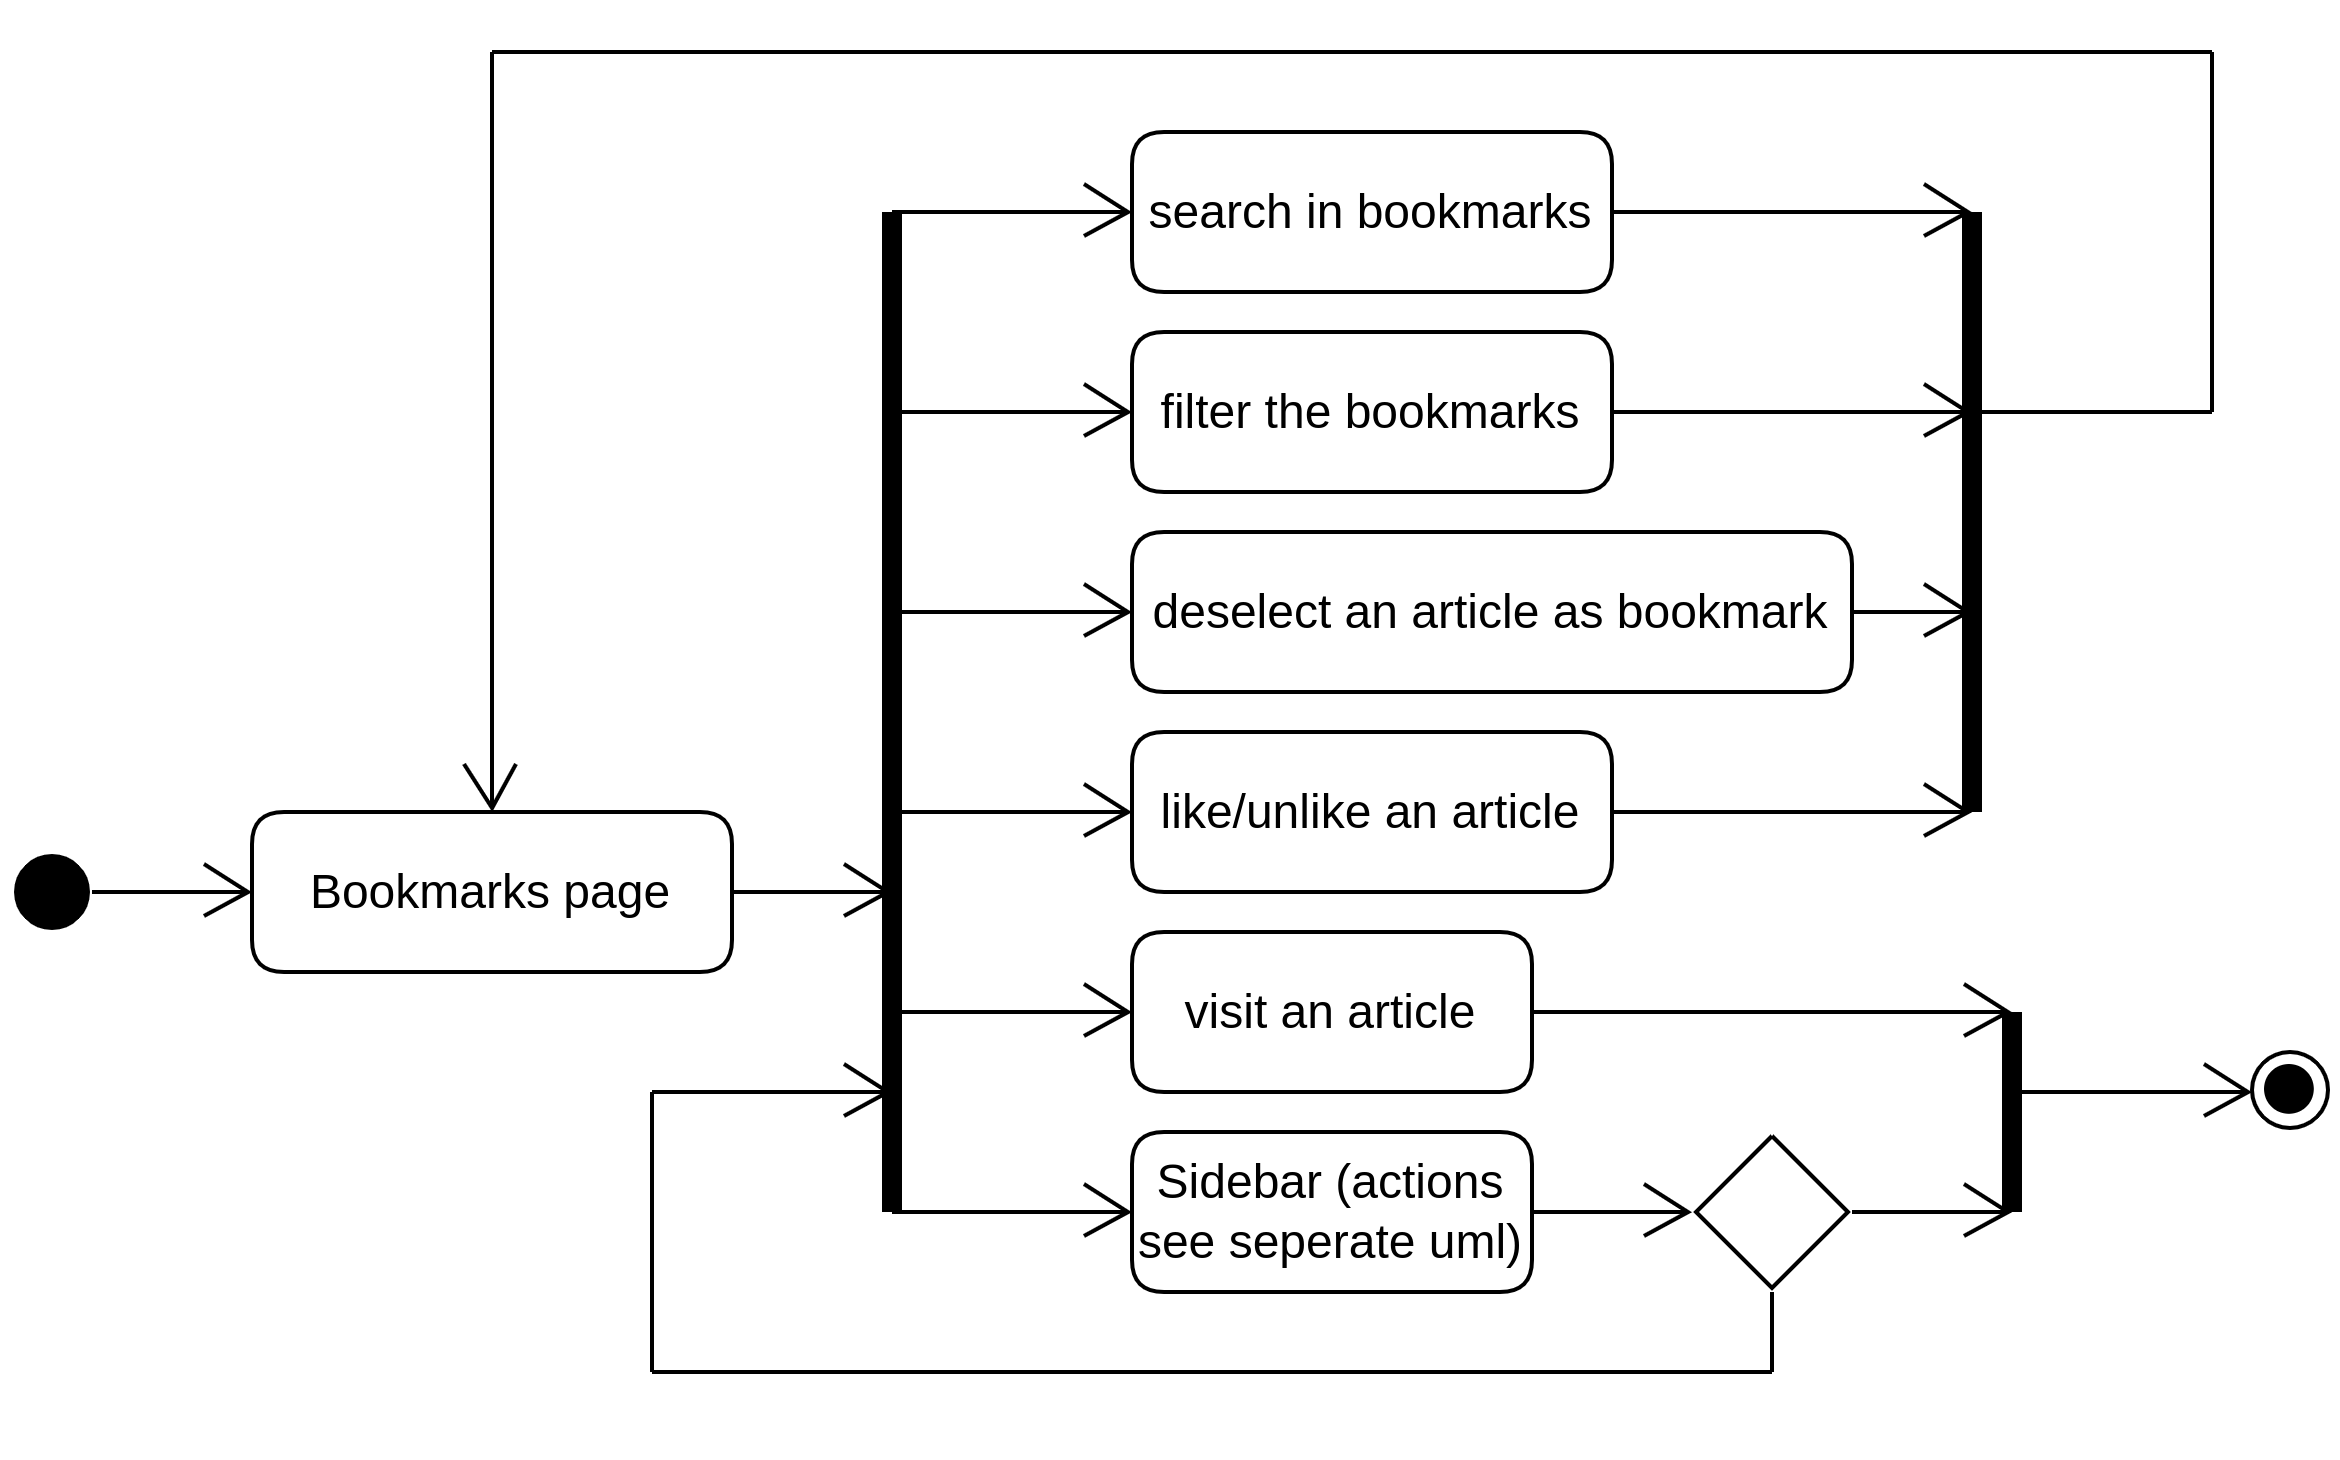
\includegraphics[width=\linewidth]{umlActivityBookmarks.png}
    \caption{Aktivitätsdiagramm der gespeicherten Lesezeichenseite}
    \label{fig:umlActivityBookmarks.png}
\end{figure}

Die Aktivitäten der Abonnementsseite werden in Abbildung~\ref{fig:umlActivitySubscription.png} abgebildet.
Die Abonnements können gefiltert und/oder durchsucht werden. Jeder Feed kann direkt deabonniert werden.
Jeder abonnierte Feed kann per Klick auf diesen aufgerufen werden.
Ein Feed kann ausgeklappt werden und die 10 aktuellsten Artikel werden angezeigt.
Die gezeigten einzelnen Artikel geliked oder als Lesezeichen gespeichert werden.

Die Artikel können mit einem Klick aufgerufen werden.
\begin{figure}
    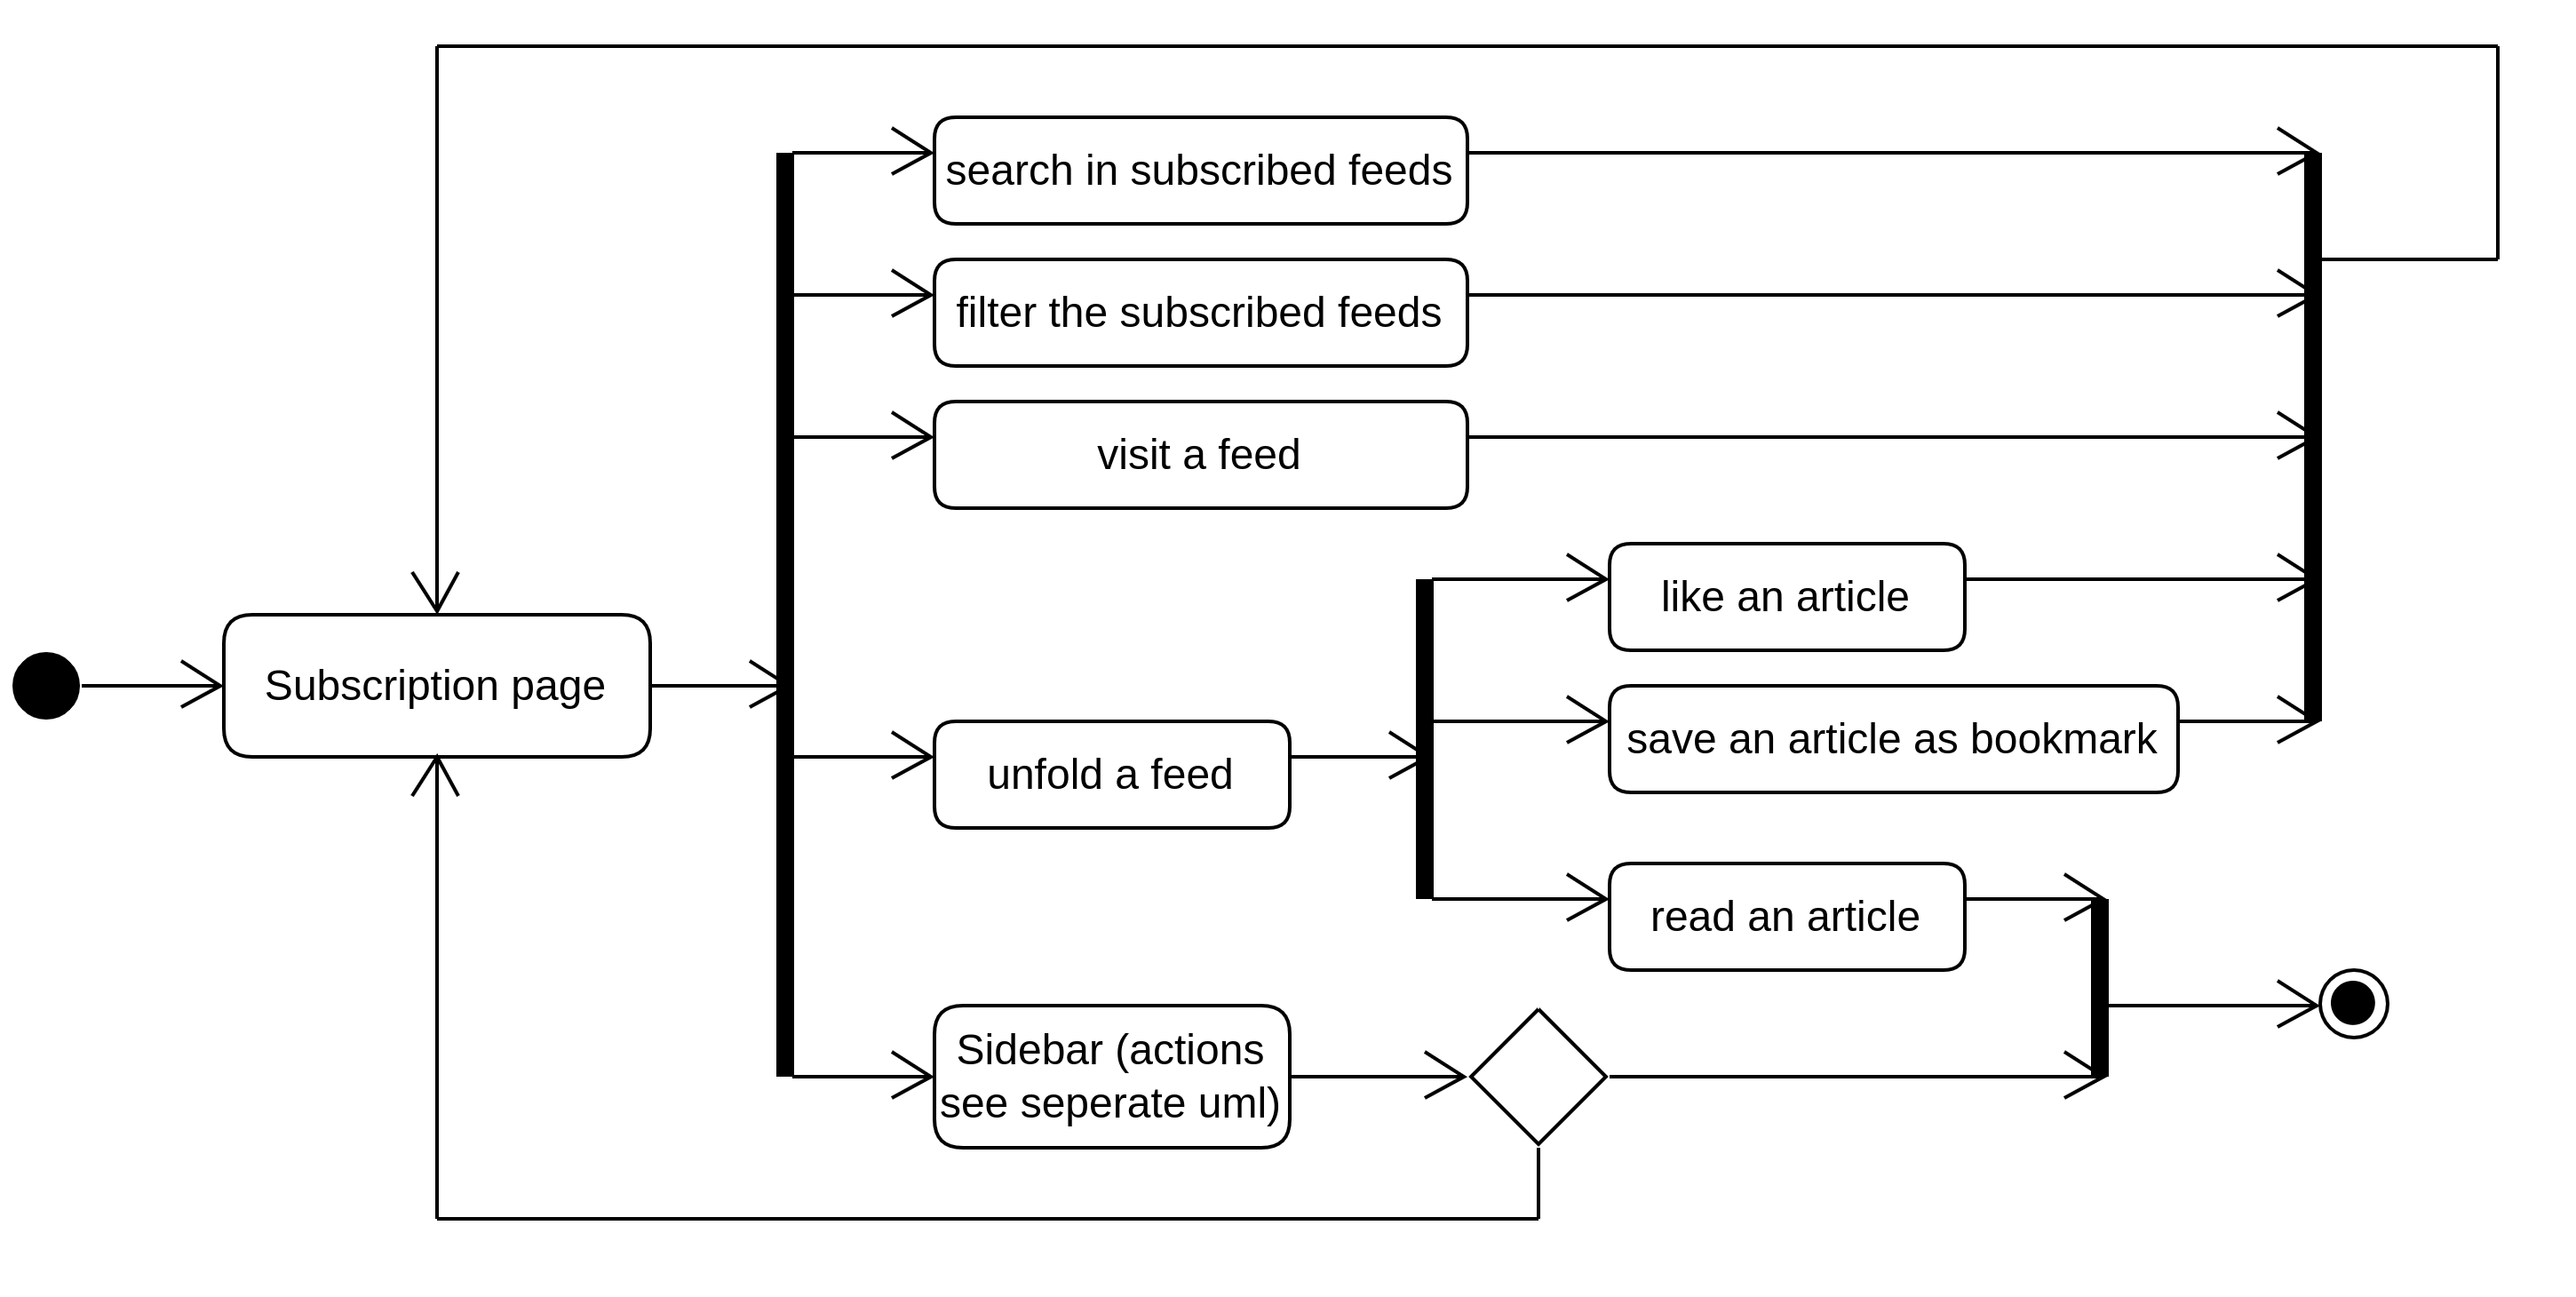
\includegraphics[width=\linewidth]{umlActivitySubscription.png}
    \caption{Aktivitätsdiagramm der Abonnements}
    \label{fig:umlActivitySubscription.png}
\end{figure}

In der Abbildung~\ref{fig:umlActivityAddFeed.png} wird der Ablauf zum Hinzufügen eines neuen Feeds dargestellt.
Ein RSS-Link wird eingetragen und mit klick auf \enquote{load} wird der Link geprüft.
Ist der Link fehlerbehaftet oder entspricht er nicht unserem Schema muss er korrigiert werden.
Funktioniert der Link werden Name und Beschreibung vorausgefüllt.
Der Name und die Beschreibung kann vor dem finalen Hinzufügen noch angepasst werden.
Das Hinzufügen eines Feeds kann jederzeit über die Schaltfläche verlassen werden.
\begin{figure}
    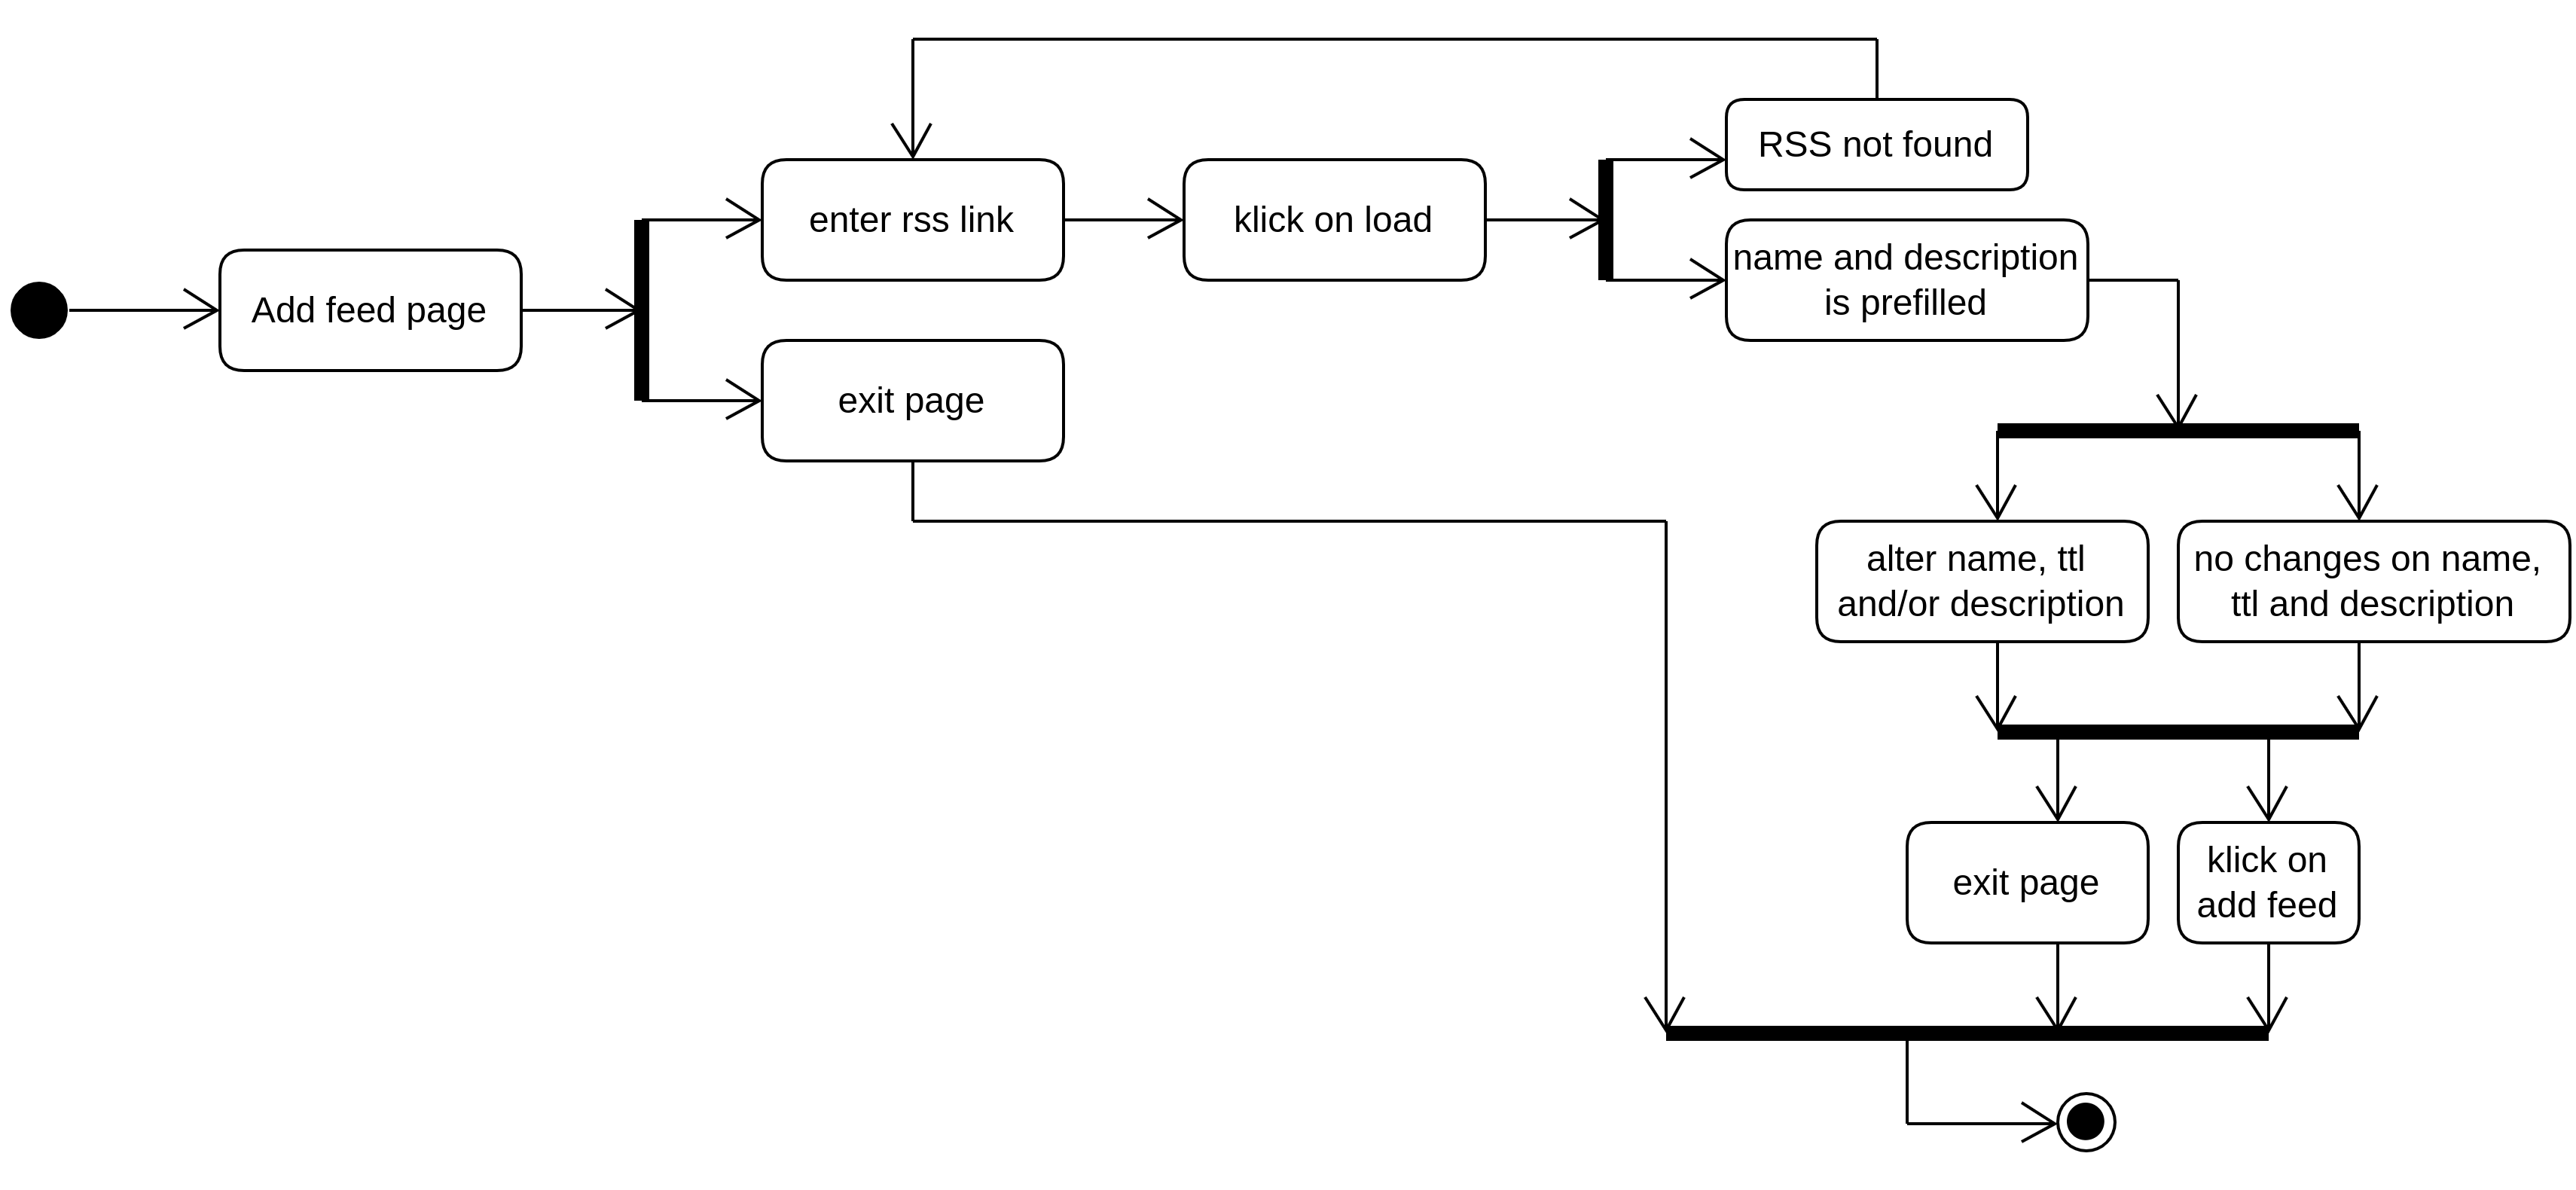
\includegraphics[width=\linewidth]{umlActivityAddFeed.png}
    \caption{Aktivitätsdiagramm zum Hinzufügen eines Feeds}
    \label{fig:umlActivityAddFeed.png}
\end{figure}

Der Nutzer kann die Einstellungen gemäß Abbildung~\ref{fig:umlActivitySettings.png} ändern.
Es können die Accounteinstellungen und das Farbschema angepasst werden.
Ausloggen kann sich der Nutzer in den Einstellungen auch.
\begin{figure}
    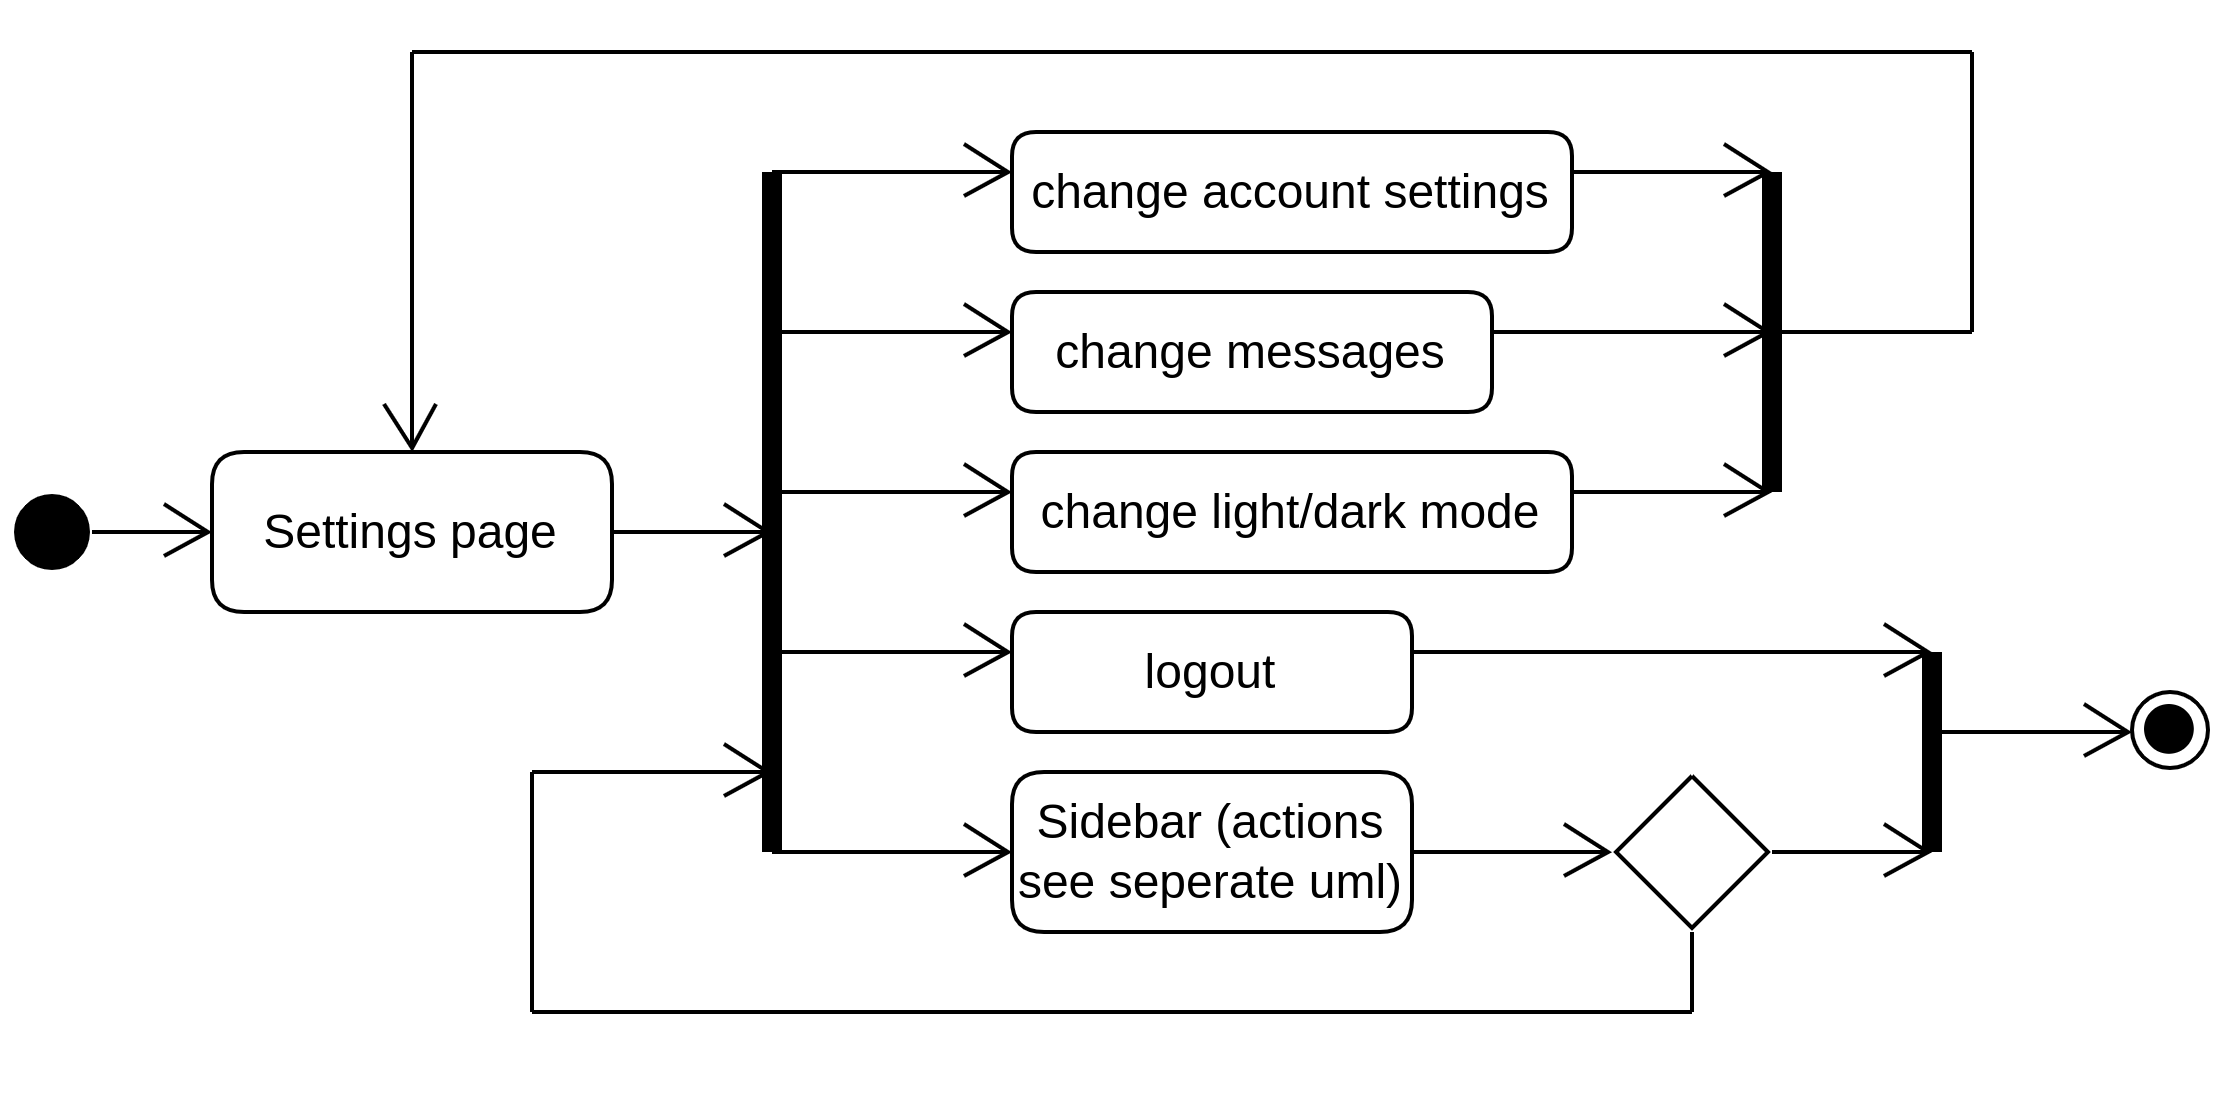
\includegraphics[width=\linewidth]{umlActivitySettings.png}
    \caption{Aktivitätsdiagramm der Einstellungsseite}
    \label{fig:umlActivitySettings.png}
\end{figure}


\section{Technische Änderungen zur anfänglichen Struktur} \label{tech_changes}
Im Laufe unseres Projektes sind einige technischen Hürden entstanden. Diese haben zum Teil dazu geführt das unsere ursprünglichen Requirements nicht mehr erfüllt werden konnten.
Deshalb wurden sie im Nachhinein dementsprechend leicht angepasst.

\begin{table}[h]
    \resizebox{\textwidth}{!}{\begin{tabular}{|p{8cm}|p{8cm}|}
    \hline
    Beschreibung der Änderung & Begründung der Änderung\\ \hline
    In der Plattform soll von RSS Feeds kein Inhalt (bzw. nur eine Beschreibung) angezeigt werden & Ein Großteil der im Internet vohandenen RSS Feeds verlinken nur auf Artikel und enthalten keinen Inhalt. \\ 
    Das Hinzufügen von Feeds aus der Creator Page wurde zu einem Must-Have Requirement & Das anfänglich geplante manuelle Einbinden von Feeds ist als zu zeitaufwändig eingeschätzt worden. \\
    Polling Intervall (TTL) nicht mehr Teil der Creator Page & Ein RSS Feed besitzt bereits ein TTL Feld, durch das dieser Interval bereits angegeben wird. \\
    \hline
\end{tabular}}
\caption{Tabelle – Änderungen zur anfänglichen Struktur}
\end{table}

Wie am Beispiel des RSS Feeds der Tagesschau\footnote{https://www.tagesschau.de/xml/rss2/} zu erkennen ist, liefern viele RSS Feeds einen TTL Wert.
Mit diesem ist zu erkennen, in welchem Intervall der jeweilige Feed neue Informationen bereitstellt. Das mögliches Polling Intervall in der Content-Creator-Page (falls implementiert) wird dadurch redundant.
Zusätzlich ist am obersten Artikel zu sehen, wie im Inhalt nur auf ein Link zur Webseite der Tagesschau verwiesen wird und nicht etwa der Inhalt des Artikels enthalten ist.
So ist es ebenfalls leicht zu erkennen, dass das Anzeigen des Inhalts, wie es in den initialen Requirements enthalten ist, nicht möglich ist.

\begin{lstlisting}[title=Tagesschau RSS Feed,language=xml]
<rss version="2.0">
    <channel>
        <title>tagesschau.de - Die Nachrichten der ARD</title>
        <link>https://www.tagesschau.de</link>
        <description>tagesschau.de</description>
        <language>de</language>
        <copyright>ARD-aktuell / tagesschau.de</copyright>
        <lastBuildDate>Tue, 03 May 2022 16:54:20 +0200</lastBuildDate>
        <docs>http://blogs.law.harvard.edu/tech/rss</docs>
        <ttl>10</ttl>
        <item>
            <title>Marktbericht: Anleger wagen sich noch etwas vor</title>
            <link>
            https://www.tagesschau.de/wirtschaft/finanzen/marktberichte/boerse-marktbericht-dax-dow-jones-101.html
            </link>
            <pubDate>Tue, 03 May 2022 18:10:20 +0200</pubDate>
            <description>
            Nach meist richtungslosem Handel kam am Ende des Tages doch noch etwas Interesse auf. Die Anleger warten derweil mit Spannung auf die Ergebnisse der Zinssitzung der US-Notenbank.
            </description>
            <guid>
            https://www.tagesschau.de/wirtschaft/finanzen/marktberichte/boerse-marktbericht-dax-dow-jones-101.html
            </guid>
            <content:encoded>
            <p> <a href="https://www.tagesschau.de/wirtschaft/finanzen/marktberichte/boerse-marktbericht-dax-dow-jones-101.html"><img src="https://www.tagesschau.de/multimedia/bilder/boerse-frankfurt-141~_v-mittel16x9.jpg"/></a> <br/> <br/> Nach meist richtungslosem Handel kam am Ende des Tages doch noch etwas Interesse auf. Die Anleger warten derweil mit Spannung auf die Ergebnisse der Zinssitzung der US-Notenbank. <a href="https://www.tagesschau.de/wirtschaft/finanzen/marktberichte/boerse-marktbericht-dax-dow-jones-101.html">mehr</a> </p> <ul> </ul> </p> <p><a href="https://www.tagesschau.de/wirtschaft/finanzen/marktberichte/boerse-marktbericht-dax-dow-jones-101.html">Meldung bei www.tagesschau.de lesen</a></p>
            </content:encoded>
        </item>
    </channel>
</rss>
\end{lstlisting}

\section{Workflows}
\subsection{Feed-Workflow}
Feeds können nur von angemeldeten Benutzer mittels unseres Frontends hinzugefügt werden. Hierfür gibt es eine Button \textit{Add Feed}, welcher ein Pop-up öffnet, in dem eine \ac{URL} zu einem \ac{RSS} Feed angegeben werden kann.
Nachdem dieser angegeben wurde, muss der Nutzer einen \textit{Load} Button betätigen, um Basis Informationen des gewünschten Feeds zu erhalten.
Falls es ein valider RSS Feed ist, werden dann die darunter liegenden Felder automatisch mit den Metadaten wie Title und Beschreibung ausgefüllt.
Dem Benutzer ist es dann möglich den Feed mit dem Button \textit{Add Feed} der Plattform hinzuzufügen.
Erst dann geschieht der eigentliche Core-Service Request, welcher versucht den angeforderten Feed abzuspeichern. Falls der Feed bereits existiert, wird eine Fehlermeldung ausgegeben.
Der Core-Service wiederum speichert den RSS Feed in der Datenbank ab. Der gesamte Workflow ist in Abbildung~\ref{fig:feedWorkflow} dargestellt.
\begin{figure}[!hbt]
    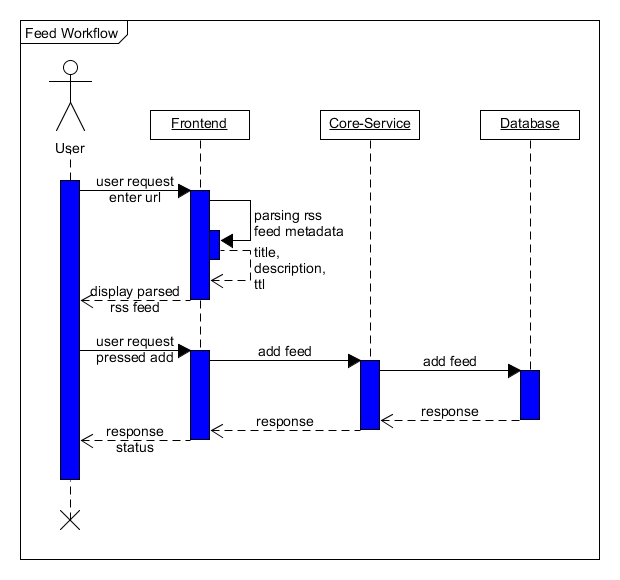
\includegraphics[width=\linewidth]{umlFeedWorkflow.png}
    \caption{Feed-Workflow}
    \label{fig:feedWorkflow}
\end{figure}

\subsection{Article-Workflow}
Mithilfe des Polling-Service werden periodisch neue Artikel-Metadaten in unsere Datenbank eingepflegt. Dieser holt sich zuerst die Feeds aus der Datenbank deren \ac{TTL} abgelaufen sind und ruft diese ab (polling).
Die dabei erhaltenen XML-Daten werden dann in ein Objekt geparst, welches weiter in unser Artikel-Objekt-Format geparst wird. Dieses enthält Informationen wie Titel, Beschreibung und einen Link zum eigentlichen Artikel.
Diese Artikel werden dann in die Datenbank eingetragen und die entsprechenden Zeitstempel der Feeds (welche zum prüfen der \acs{TTL} verwendet werden) geupdated.

Besucht ein Nutzer unsere Startseite oder eine Artikel-Seite wird vom Frontend eine Anfrage an das Backend (Core-Service) gestellt, um Artikel zu erhalten. Dieses holt sich Artikel aus der Datenbank und gibt explizit
angefragte Artikel sowie Empfehlungen für weitere Artikel an das Frontend zurück. Das Frontend stellt dem Nutzer dann die Artikel(-empfehlungen) dar. Der gesamte Workflow ist in Abbildung~\ref{fig:articleWorkflow} dargestellt.

\begin{figure}[!hbt]
    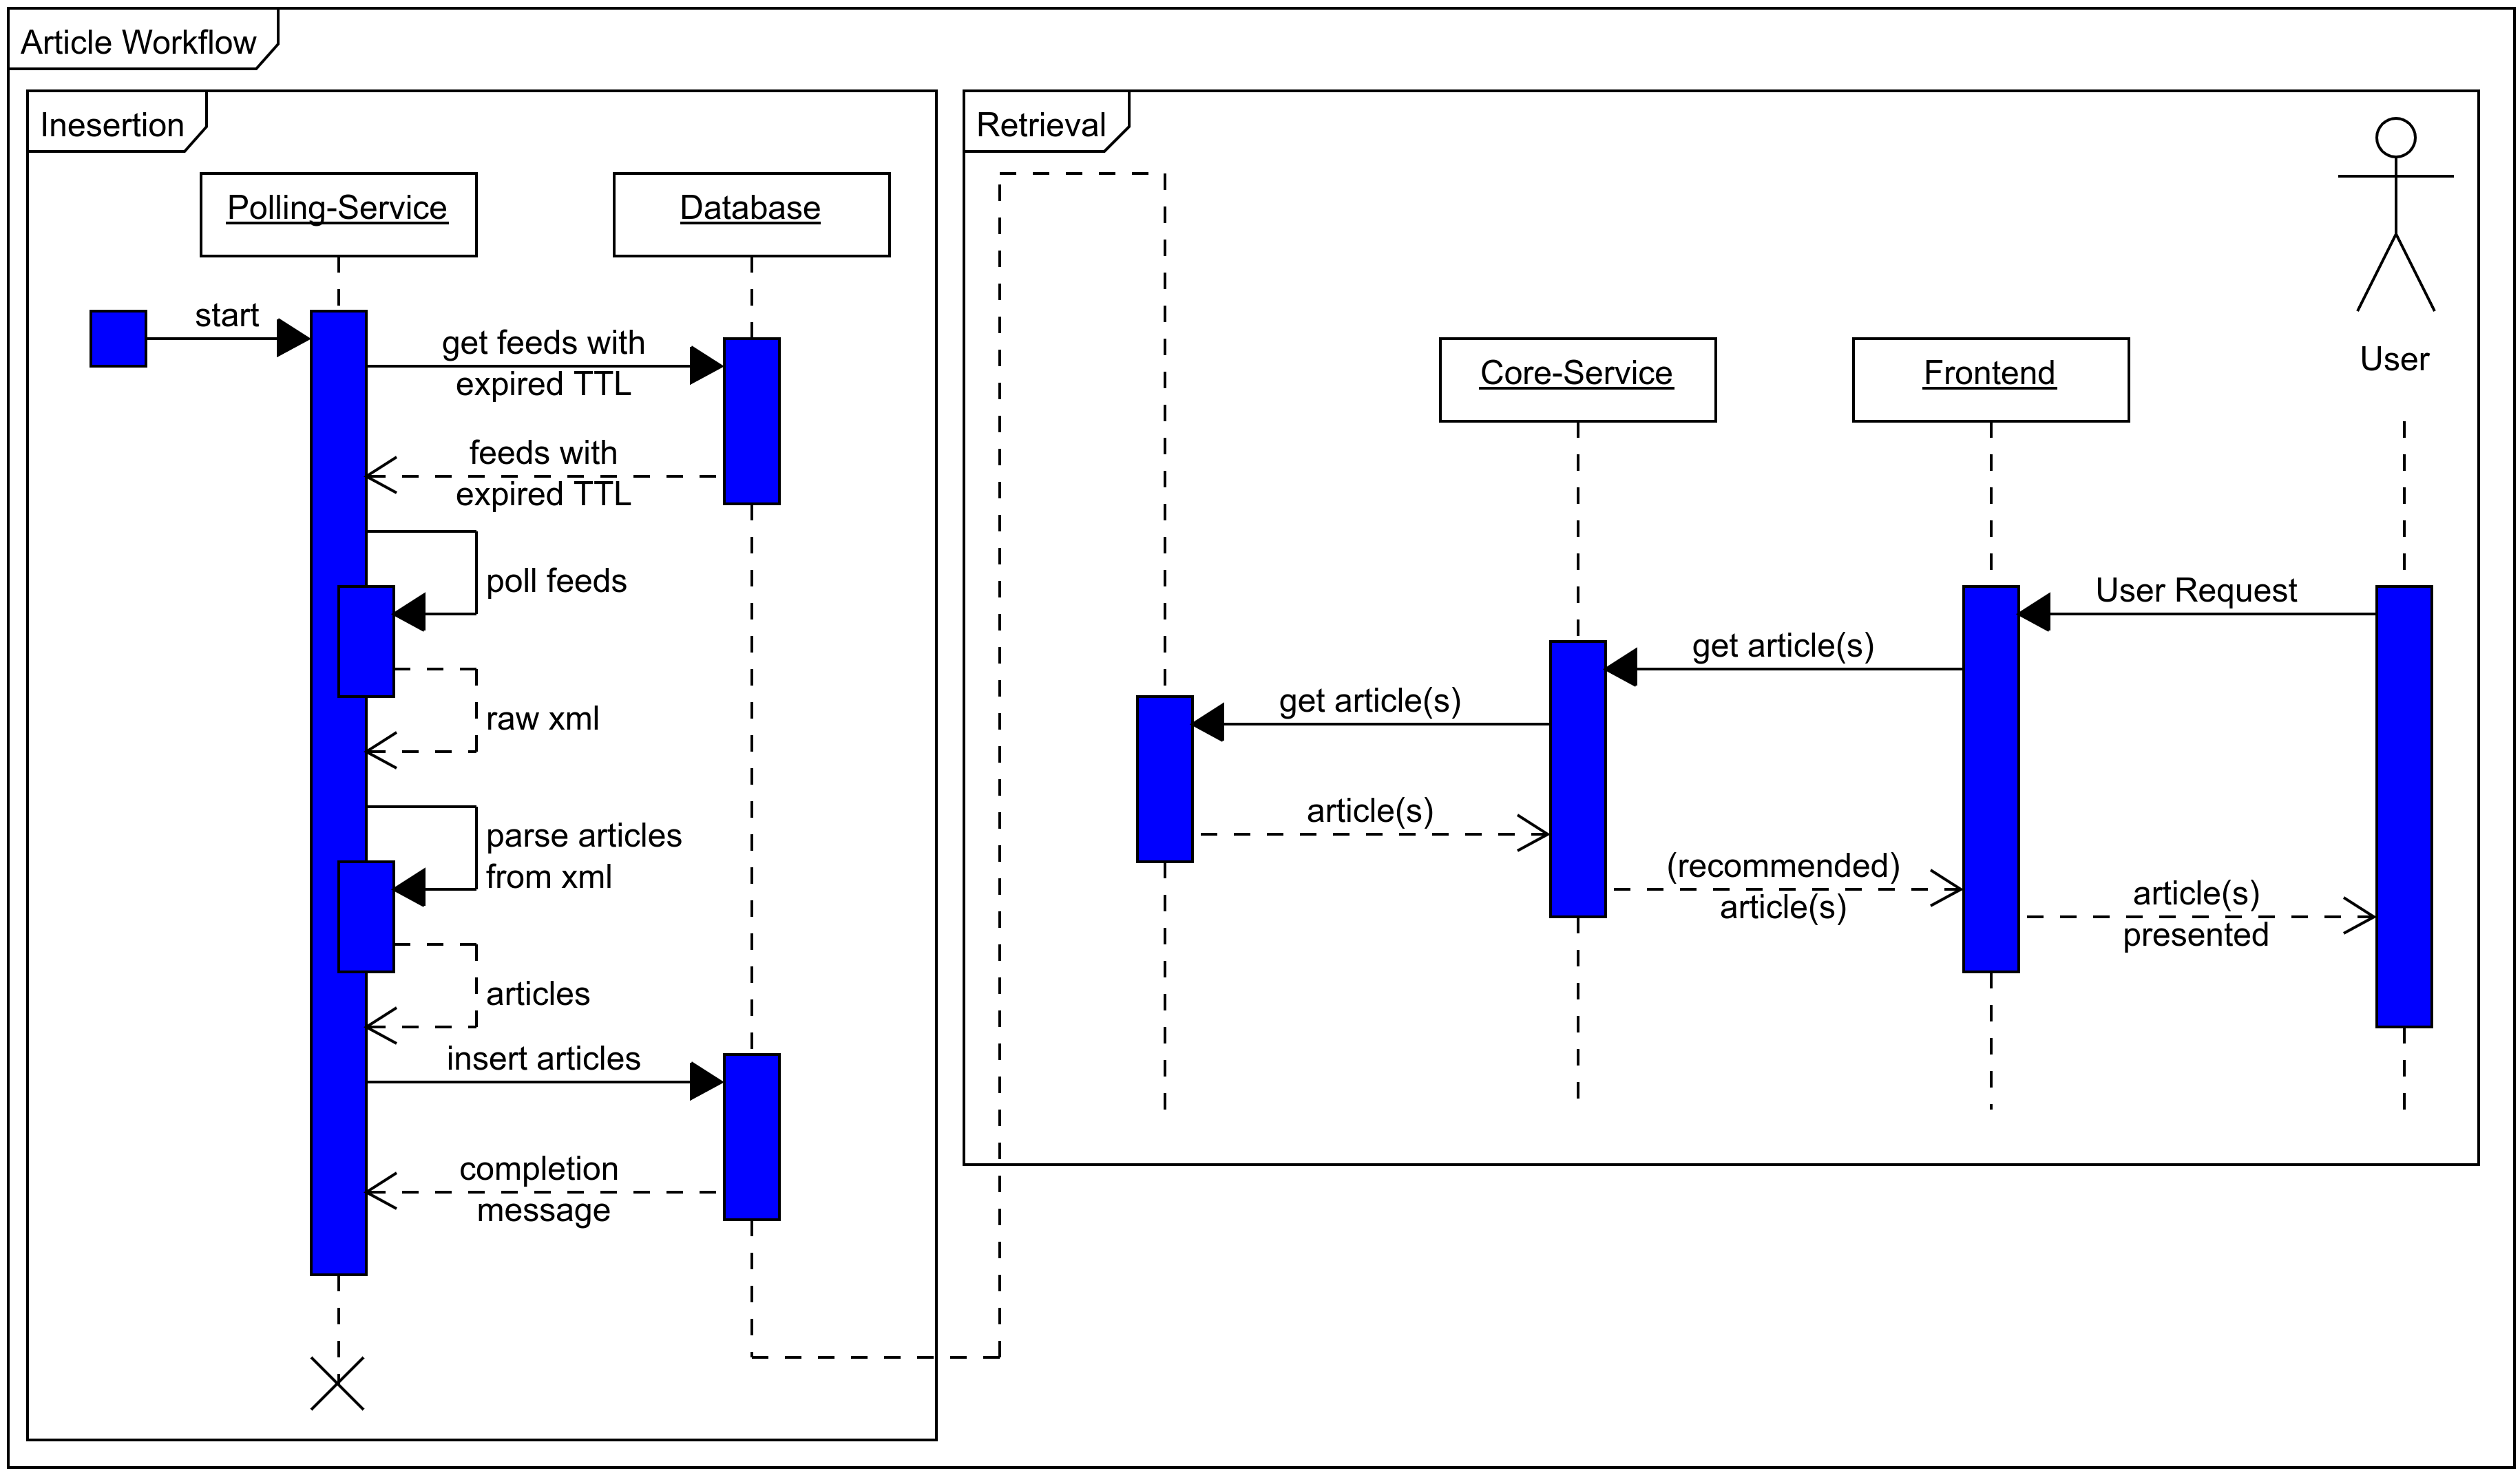
\includegraphics[width=\linewidth]{umlArticleWorkflow.png}
    \caption{Artikel-Workflow}
    \label{fig:articleWorkflow}
\end{figure}
